\documentclass[a4paper,11pt]{article}
\pdfoutput=1 % if your are submitting a pdflatex (i.e. if you have
             % images in pdf, png or jpg format)
\usepackage{jheppub} % for details on the use of the package, please
                     % see the JHEP-author-manual
\usepackage[T1]{fontenc} % if needed

\usepackage{wrapfig,lipsum,booktabs}
\DeclareMathAlphabet{\scr}{U}{rsfs}{m}{n}
\usepackage{latexsym}
\usepackage{epsfig}
\usepackage[mathscr]{eucal}
\usepackage{amsfonts}
\usepackage{amscd}
\usepackage{amsmath}
\usepackage{array}
\usepackage{amssymb}
\usepackage{colordvi}
\usepackage{enumerate}
\usepackage{graphicx}
\usepackage{booktabs}
\usepackage[footnotesize]{caption}
\usepackage{fancyhdr} 
\usepackage{pdfpages}
\usepackage{slashed}
\usepackage{tabularx}
\usepackage{longtable}
\usepackage{array}
\usepackage{relsize}
\usepackage{color}
\usepackage{rotating}
\usepackage{slashed}
\usepackage{subfigure}
\usepackage{xspace}
\usepackage{booktabs}
\usepackage{epsfig,amsmath,graphicx,amssymb,listings,slashed}
\usepackage[colorlinks,citecolor=blue,urlcolor=blue,linkcolor=blue]{hyperref}


\title{{\boldmath Extending the pMSSM Coverage with Gluino-Squark \\ Simplified Models Results}}


%% %simple case: 2 authors, same institution
%% \author{A. Uthor}
%% \author{and A. Nother Author}
%% \affiliation{Institution,\\Address, Country}

% more complex case: 4 authors, 3 institutions, 2 footnotes
\author[a,]{Federico Ambrogi,\note{Corresponding author.}}


% The "\note" macro will give a warning: "Ignoring empty anchor..."
% you can safely ignore it.

\affiliation[a]{Department of Meteorology and Geophysics, University of Vienna, Vienna, Austria}


% e-mail addresses: one for each author, in the same order as the authors
\emailAdd{federico.ambrogi@univie.ac.at}


%% ---------------------------------
%% | New commands                  |
%% ---------------------------------
\newcommand{\MET}{{ $E_T ^{miss}$}}

\newcommand{\amc}{{\sc MadGraph5\textunderscore}a{\sc MC@NLO}}
\newcommand{\pyE}{{\sc Pythia\,8}\xspace}
\newcommand{\pys}{{\sc Pythia\,6}\xspace}
\newcommand{\pythiaS}{{\sc Pythia\,6}\xspace}
\newcommand{\pythiaSF}{{\sc Pythia\,6.4}\xspace}

\newcommand{\nllfast}{{\sc NLLfast}\xspace}
\newcommand{\delphes}{{\sc Delphes\,3\xspace}}

\newcommand{\MA}{\texttt {MadAnalysis5\xspace}}
\newcommand{\SMO}{\texttt{SModelS\xspace}}

\newcommand{\MSQ}{$ m _{ \tilde q } $\xspace} 
\newcommand{\MGLU}{$ m _{ \tilde g } $\xspace} 
\newcommand{\WEIGHT}{$\sigma \times BR$\xspace} 
\newcommand{\RVALUE}{\textit{r value}} 

\newcommand{\FASTLIM}{\texttt{FastLim}} 

\newcommand{\TGQ}{ \textit{T3GQ}} 
\newcommand{\Tone}{ \textit{T1}} 
\newcommand{\Ttwo}{ \textit{T2}} 
\newcommand{\Tfive}{ \textit{T5}} 





\abstract{After the Run 1, where proton-proton collisions were performed at the Large Hadron Collider (LHC) at 8 TeV centre-of-mass energy, the ATLAS collaboration analysed the constraints on a 19-parameters realisation of the phenomenological Minimal Supersymmetric Standard Model (pMSSM) using the results of the many searches for new physics. A large portion of the parameter space excluded by the ATLAS collaboration can also be efficiently constrained using directly the simplified model results, which became the standard method employed for the interpretation of searches for Beyond the Standard Model (BSM) physics. Moreover the still uncovered part could be potentially covered by a new class of simplified model stemming from gluino-squark associated production, producing a 3 jets plus missing energy signature in the LHC detectors. This work aims at demonstrating that by recasting existing searches with such simplified model, it is possible to extend significantly the coverage of the pMSSM-19 parameter space by means of simplified models results, and avoid the computationally expensive procedure of analysis recasting.}
\begin{document} 
\maketitle
\flushbottom
\section{Introduction}
Simplified models spectra (SMS) have become the standard method for the LHC collaborations to interpret the results of their searches for Beyond the Standard Model (BSM) particles, as in the case of Supersymmetry (SUSY). The most notable benefit is the drastic reduction of the large parameter spaces of full theories to a handful of new states. SMS serve not only as a useful benchmark to design and optimize the searches, but also they can easily highlight the specific strength of each search. Only a few SUSY particle appears in each SMS, while all the remaining SUSY particles are too massive to be produced at the LHC energy due to very small cross section production, and they can not appear as intermediate on-shell states in cascade decays. 
\\
In the case of SUSY, the masses of the of the particles, their production cross section and their decay modes are sufficient to fully characterise each SMS. Once these parameters are fixed, it is straightforward to estimate the exclusion provided by the LHC searches with SMS. The interpretation of searches with SMS started back at the early LHC era, with the data collected at a centre-of-mass energy of 7 TeV (see e.g. \cite{Chatrchyan:2013sza} by the CMS Collaboration). The choice of specific SMS relies on their simple experimental signatures and kinematical properties of the particles captured by the detectors. It is to be particularly stressed how the kinematics of the events is determined mainly by the mass scale of the SUSY particles involved, rather than the specific quantum or gauge numbers of the theory. Using SMS to re-interpret the results  of  the searches in the context of complete theory is however challenging. The main difficulty comes from considering the full particle spectra appearing in general theories. In fact, considering for example the R-parity conserving MSSM, the kinematics of the cascade decays to the lightest supersymmetric particles (LSP) might differ significantly from the on of the simplified case. The SMS commonly used for the interpretation of searches normally include up to three SUSY particles masses for cascade decays, or for asymmetric production (production of two different SUSY particles).


For the task of re-interpretation of searches with SMS results, 
dedicated tools such as \FASTLIM \cite{Papucci:2014rja} and \SMO \cite{Kraml:2014sna} were developed. They can decompose the signal of SUSY models into its SMS, and check the constraints provided by the LHC searches, contained in a dedicated database of results. In particular, \SMO~ was used in \cite{Ambrogi:2017lov} to study the coverage of the pMSSM-19\cite{Djouadi:1998di} with SMS with respect to the full recast analyses performed by the ATLAS collaboration. Specifically, the set of pMSSM points considered were made public by the ATLAS collaboration on the \texttt{HepData} website\cite{ATLASpMSSMhepdata}. The sensitivity of the ATLAS searches for a selection of BSM searches on the pMSSM was presented in \cite{Aad:2015baa}. They re-run their analyses on thousands of pMSSM model points, and characterised the constraints offered by each search considered for the reinterpretation .
%
\\
The same model points were then tested with \SMO~ v1.1\cite{Ambrogi:2017neo}, obtaining a total coverage of roughly 55$\%$-63$\%$ for the Bino and Higgsino-like LSP case, respectively\footnote{The Wino-like LSP dataset was neglected since most of the model pointed included long-lived charged particles, a signature which could not be handled by the v1.1 used.}. The work also showed that by means of efficiency maps (EM) results, that can be produced by phenomenologists outside the experimental collaborations, it was possible to increase significantly the number of excluded point. This is mainly due to the fact that the LHC collaborations provide results only for a limited set of SMS, and many interesting model, to which existing searches are sensitive to, are left unexplored.
\\
Indeed, the comparison between the \SMO~ approach and the re-interpretation performed by the ATLAS collaboration showed  that the main limitation of the simplified model approach is the lack of results for simple signatures, such as the $3jets$ + missing energy (\MET). One of the \SMO~ tool main features is the ability of extracting the most relevant signatures in terms of $\sigma \times BR$ (production cross section  times branching ratio) that are not currently constrained by simplified models results, called \textit{missing topologies}. The aforementioned $3jets$ +\MET~ signature can arise, for example, from gluino-squark associated production, where the gluino decays preferentially to an on-shell lighter squark, in turn decaying to a quark (that is reconstructed by the analysis as a jet of hadrons) and the LSP. This simplified model can be fully described by three mass parameters of the sparticle involved: $m_{\tilde g}, m_{\tilde q}$ and $m_{\tilde \chi _1 ^0}$. However, under the simplified model assumption, results for such model can be used to constrain the alternative mass hierarchy where the squark is heavier than the gluino, so that in this scenario the squark decays to on-shell gluino. The gluino can then decay radiatively to a gluon and the LSP or via an off-shell squark (i.e. 3-body decay, producing a $4jets$ + $E_T ^{miss}$ signature), depending on its mass difference with the lightest squark. 
The idea at the basis of this paper is to extend the previous study of the coverage of the pMSSM, and concretely show how the inclusion of newly created EM for the $3jets$ + \MET~signature increases the coverage of the pMSSM. This can be efficiently done by combining the information obtained with \SMO~ regarding the important missing topologies, and the usage of analyses recasting tools to produce EMs results for arbitrary simplified models, to be implemented in the database of experimental results. For this purpose, this paper is structured as follows. Section \ref{sec::T3GQ} summarises the main characteristics of the $3jets$ + \MET~signature arising from gluino-squark production. In Section \ref{sec::setup} the set up of the \SMO~ analysis is described: the details regarding the production of the EMs for the gluino-squark model are discussed, and the set of pMSSM points used for the study are provided. Section \ref{sec::impact} summarises the improved constrained obtained with the newly added EMs, in particular discussing the benefit of the signal combination from EM results. A brief analysis of the current state of the art simpliifed model results at 13 TeV is discussed in Chapter \ref{ch::13TeV}. Finally an outlook about future extensions of the procedure is given in the conclusive Chapter \ref{sec:conclusion}.  
%
\section{The 3 jets + $E_T ^{miss}$ Signature }\label{sec::T3GQ}
\begin{figure*}
	\begin{center}
		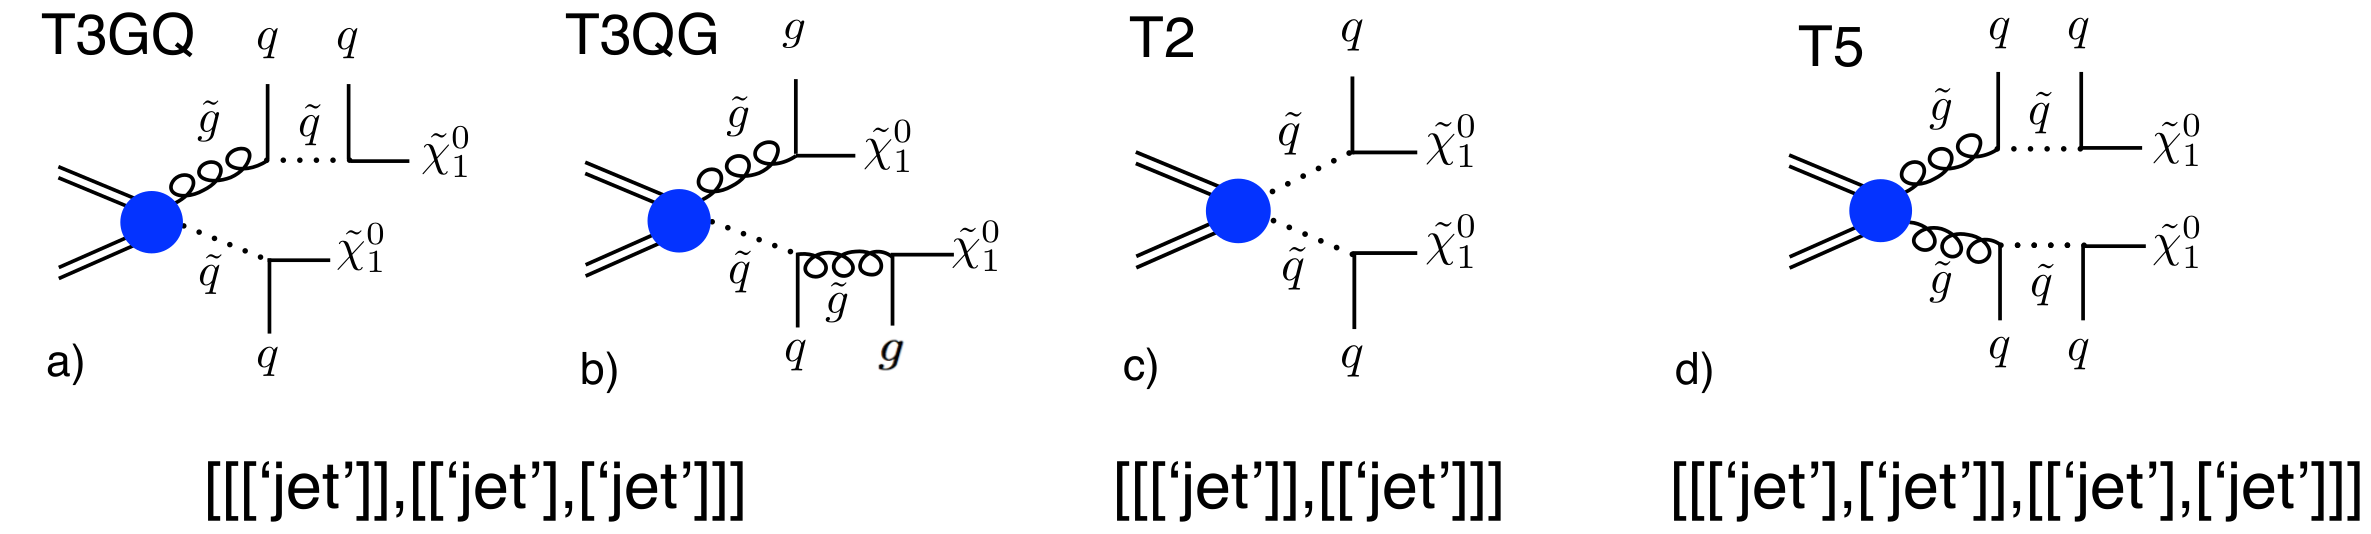
\includegraphics[width=0.95\textwidth]{PLOTS/diagrams.png}
	\end{center}
	\caption{Diagrams for the simplified models used for the extension of the database. Models \textit{T3GQ}(a) and \textit{T3QG}(b), corresponding to the two different mass hierarchies $m_{\tilde g} > m_{\tilde q}$ and $m_{\tilde q} > m_{\tilde g}$, are identified by the experimental signature \textit{[[[`jet']],[[`jet’],[`jet']]]} in \SMO~ notation. Light quarks and gluons are included in the definition of `jet'. Diagrams c) and d) represent the \textit{T2} and \textit{T5} models, mapping to the \textit{[[[`jet’]],[[`jet']]]} and \textit{[[[`jet’],[`jet']],[[`jet’],[`jet']]]} signatures. Note that the insertion of the final state particles in the vertices of each topology uniquely identifies a given simplified model.}
	\label{Diagrams}
\end{figure*}
In generic pMSSM-19 points, the squark mass parameters are: 
\begin{equation*}
m_{\tilde u_L} = m_{\tilde d_L} = m_{\tilde c_L} = m_{\tilde s_L} 
\end{equation*}
\begin{equation*}
m_{\tilde u_R} = m_{\tilde c_R} 
\end{equation*}
\begin{equation*}
m_{\tilde d_R} = m_{\tilde s_R}
\end{equation*}
\\
Since the mass of the gluinos is another free parameter, there are two possible mass hierarchies of interest. 
When considering for simplicity the lightest of the squark masses with $m_{\tilde g} > min(m_{\tilde q})$ (and the other third generation squark set to a high scale), gluino will decay almost entirely to an on-shell intermediate squark, followed by the decay of the squark to the LSP:
\begin{equation}\label{decay_TGQ}
p p \rightarrow \tilde g \tilde q , \tilde g \rightarrow \tilde q q , \tilde q \rightarrow q \tilde \chi_1 ^0
\end{equation}
\\
However, for the alternative hierarchy where the squark considered is heavier than the gluino,  $ min(m_{\tilde q}) > m_{\tilde g}$ the squarks will decay to an on-shell intermediate gluino. The gluino will then decay either via radiative decay to the LSP as 
\begin{equation}\label{decay_loop}
p p \rightarrow \tilde g \tilde q ,\tilde q \rightarrow \tilde g q , \tilde g \rightarrow g \chi_1 ^0
\end{equation} 
\\
or, for small $\Delta M(min(m_{\tilde q}), m_{\tilde g})$,  via a three-body decay from off-shell squark:
\begin{equation}
p p \rightarrow \tilde g \tilde q ,\tilde q \rightarrow \tilde g q, \tilde g \rightarrow q \bar q \tilde \chi _1 ^0.
\end{equation}
\\
The simplified model of interest of this work produces a $3jet$ + missing energy final state as formulated in the Decays \ref{decay_TGQ} and \ref{decay_loop}\footnote{Both correspond to the \textit{[[[`jet']],[[`jet'],['jet']]]} signature in the \SMO~ bracket language.}. This experimental signature can be obtained by considering two different mass hierarchies, which are depicted by the diagrams a) and b) in Fig. \ref{Diagrams}. The first, labelled \textit{T3GQ} represents the case where the gluinos are heavier than the squarks considered; the latter, labelled \textit{T3QG} represents the alternative case. Note that for our purposes, it is sufficient to consider only the lightest of the three squarks. Depending on the specific pMSSM model point considered, one of the two alternative mass hierarchies will produce this specific signature, due to the strong nature of the gluino-squark coupling.
%
As stated in the introduction, the \textit{T3GQ} model was found to be the most important missing result for the pMSSM. It is to note, however that, by construction, the \textit{T2} and \textit{T5} models, represented by plots c) and d) of Fig. \ref{Diagrams}, are automatically important when the \textit{T3GQ} model also is. In practice, the \textit{T3GQ} model is an asymmetric model composed by one branch from the \textit{T2} and one branch from the \textit{T5} models. Thanks to the usage of EM results, it is thus possible to combine the signals from the $pp \rightarrow \tilde g \tilde g$, $pp \rightarrow \tilde q \tilde q$ and $pp \rightarrow \tilde g \tilde q$ channels. Along with the results from \textit{TGQ}, the power of combining the \textit{T2} and \textit{T5} models will be explored in this work. For completeness, results for the \textit{T2} and \textit{T5} models were already included in the previous release of the database, hence did not appear in the missing topologies list of the original study. 
\section{Production of the Efficiency Maps}\label{EMprod}
The set-up for the production of the Monte Carlo signals is the following. Events at parton level were generated using \texttt{MadGraph5\_aMC@NLO}\cite{Alwall:2011uj}, and then showered and hadronized using \texttt{Pythia 6.4}\cite{Sjostrand:2006za}. The processes considered for the production of the samples for the simplified model are described in Tab. \ref{mg5_processes}.


\begin{wraptable}{r}{8cm}
	\small
	\begin{center}
		\renewcommand{\arraystretch}{1.0}
		\begin{tabular}{ l l }  \toprule  \toprule 
			%\multicolumn{3}{c}{($M_1,M_2,M_3) = (1000,200,190)$} & \multicolumn{3}{c}{ \textbf{T3GQ}} & \multicolumn{3}{c}{ \textbf{T3QG}} \\  \toprule 
			\multicolumn{2}{c}{\texttt{MadGraph5\_aMC@NLO} processes} \\ \toprule \toprule
			\multicolumn{2}{l}{\Ttwo: $p p \rightarrow \tilde q \tilde q$}  \\
			& define Q = dl dr dl\textasciitilde dr\textasciitilde ul ur ul \textasciitilde ur\textasciitilde \\
			& generate p p $>$ Q Q  \\
			&  add process p p $>$ Q Q j \\  \toprule 
			\multicolumn{2}{l}{\Tfive: $p p \rightarrow \tilde g \tilde g$ } \\ 
			& generate p p $>$ go go \\
			&  add process p p $>$ go go j \\ \toprule 
			\multicolumn{2}{l}{\TGQ: $p p \rightarrow \tilde g \tilde q$} \\  
			&  define Q = dl dr dl\textasciitilde dr\textasciitilde ul ur ul\textasciitilde ur\textasciitilde \\
			&  generate p p $>$ go Q \$ go Q \\
			&  add process p p $>$ go Q j \$ go Q \\  \bottomrule \bottomrule 
			%
		\end{tabular}
	\end{center}
	\normalsize
	\caption{\texttt{MadGraph5\_aMC@NLO} processes for the production of the Monte Carlo samples.}
	\label{mg5_processes}

\end{wraptable}
Note that the processes considered the emission of up to one extra parton. The syntax $\$go \ Q$ is used to avoid the presence of on-shell resonances, represented by intermediate gluino or squarks, that would lead to double counting when performing the merging between matrix-element and parton-shower. The merging between the matrix elements and parton-shower formalisms was performed adopting the $k_T \ jet$ MLM scheme \cite{MLM,Alwall:2007fs}. 
%
The analysis recasting was performed with \texttt{MadAnalysis 5}, using the recasting codes for the analysis ATLAS-SUSY-2013-02\cite{ATLAS-SUSY-2013-02MA5,ATLAS-SUSY-2013-02VALIDATION} and CMS-SUS-13-012\cite{CMS-SUS-13-012MA5,CMS-SUS-13-012VALIDATION}. The tuned version of \texttt{DELPHES 3} integrated in the \texttt{MadAnalysis 5} framework was used to take into consideration the detector efficiency on the particles. Jets were clustered using \texttt{FastJet}\cite{Cacciari:2011ma}.
%
The description of the grid of mass points defined for the production of the efficiency maps is provided in Tab. \ref{TGQ_Planes}. The analyses chosen for the recasting search for SUSY events in the all hadronic final state, vetoing the presence of isolated leptons. In particular the two above analyses are sensitive to events with small jet multiplicity, as generated by the simplified models considered. Although official EM results for the \textit{T2} model were made public by the collaborations, part of the parameter space with small mass gap between the squark and the LSP is below $~$50 GeV is not properly covered. For this reason, EMs were produced to replace the official results, up to a mass difference as small as 5 GeV between the squarks and the LSP. In addition, also the results for the \Tfive~model were extended to cover scenarios with small mass difference between the gluino-squark and squark-LSP. The parameter $x$ is defined so that
\begin{equation}
m_{\tilde q}= x\cdot m_{\tilde g} + (1-x)\cdot m_{\tilde \chi_1 ^0}.
\end{equation}
%
For the \textit{T3GQ} model, the gluino mass reaches the value of 2 TeV, with a binning of 50 GeV for $200 \leq m_{\tilde g} < 1200$, and a binning of 100 GeV for $1200 \leq m_{\tilde g}  \leq 2000$ GeV. The squark masses for the \textit{T3GQ} have a 50 GeV binning, and reach the maximum value of 1 TeV. For a better coverage of the parameter space in the case of small mass differences, additional mass planes parametrized with 
\begin{equation}
\Delta M ( \tilde q, \tilde \chi _1 ^0)=(5,10,15) \ GeV
\end{equation}
were produced. Note that the values of the maximum values of the gluinos and squarks were chosen arbitrarily, since a priory there is no possibility to determine the efficiency of the analysis and of the cross section upper limit. It will be see in Section \ref{sec::impact} that indeed this limit should be extended to regions of larger \MGLU, since both the efficiency of the recast analyses considered and the associated gluino-squark production cross sections are sufficiently sizeable.
%

\begin{wraptable}{r}{8cm}
	\footnotesize
	\begin{center}
		\small
		\renewcommand{\arraystretch}{1.0}
		\begin{tabular}{ l l l }  \toprule \toprule 
			\multicolumn{3}{c}{\texttt{ \normalsize \textbf{Mass Planes}}} \\ \toprule \toprule
			\multicolumn{3}{l}{\Ttwo: $p p \rightarrow \tilde q \tilde q$} \\
			& - & min($\Delta M(\tilde q, \tilde \chi _1 ^0)$) = 5 GeV \\ \midrule
			\multicolumn{3}{l}{\Tfive: $p p \rightarrow \tilde g \tilde g$} \\ 
			&x=(0.05,0.50,0.95) &  \\ 
			&$\Delta M(\tilde q, \tilde \chi _1 ^0)$ = 5 GeV&  \\ \midrule
			\multicolumn{3}{l}{\TGQ: $p p \rightarrow \tilde g \tilde q$} \\  
			& $m_{\tilde g}$ = 200,...,1200 & 50 GeV bin \\ 
			& $m_{\tilde g}$ = 1300,...,2000 & 100 GeV bin ($m_{\tilde g}\leq$2 TeV) \\
			& $m_{\tilde q}$ & 50 GeV bins ($m_{\tilde q}\leq$1 TeV) \\
			& & min($\Delta M(\tilde q, \tilde \chi _1 ^0)$) = 5 GeV \\ \bottomrule \bottomrule
		\end{tabular}
	\end{center}
	\normalsize
	\caption{Mass plane parametrization used for the EMs production of the \textit{T2}, \textit{T3GQ} and \textit{T5}. See the text for details.}
	\label{TGQ_Planes} 
\end{wraptable}
%
For the gluino-squark model we chose the hierarchy $m_{\tilde g} > m_{\tilde q}$, so the \textit{T3GQ} model was chosen to constrain the "[[[`jet']],[[`jet],[`jet']]]" signature. Note that the same problem related to the choice of the mass hierarchy applies to the $T5$ model: the "[[[`jet']],[[`jet']]]" signature can be obtained both with $\tilde g \rightarrow g \tilde \chi _1 ^0$ and $\tilde q \rightarrow q \tilde \chi _1 ^0$. Also for the recasting of this model the former hierarchy was chosen. In \ref{app:ul} the comparison between the values of the upper limits and efficiencies obtained for the two different mass hierarchy, for two benchmark points, are provided. Differences can indeed arise due to the different hadronization and clustering of quarks and gluon into jets, so that the jets momentum and multiplicity, and linked kinematics variables such as the hadronic transverse energy, might differ. However such differences have a limited impact in the efficiency selection, typically contained within 20$\%$. The observed UL calculation, however, is based on the selection of best expected signal region, i.e. the signal region which provides the best expected limit. The observed number of events indeed suffer from statistical fluctuation, that might be quite different from one signal region to another. For this reason, a small difference in the efficiency might lead to the selection of a different signal regions providing the best expected limit, and consequently to a discording observed UL from SR to SR. While this might result in up to a factor 2 difference in the observed UL, this translates into a modest uncertainty in the cross section UL and in the mass of the related SUSY particle, with little impact in the general interpretation of the excluded regions of the parameter space of the tested pMSSM-19. 
%
It is important to stress that \SMO~ does not distinguish between gluon and light quarks in the final states, both generically identified as "jet". This happens with the \TGQ~model as seen explicitly in diagrams a0 and b) of Fig. \ref{Diagrams}, where both quark and gluon jets appear. Consequently also also the \Ttwo~and\Tfive~results can be used to constrain the alternative models $p p \rightarrow \tilde g \tilde g ,\tilde g \rightarrow \tilde g \chi _1 ^0$ and $p p \rightarrow \tilde q \tilde q ,\tilde q \rightarrow \tilde g q, \tilde g \rightarrow g \tilde \chi _1 ^0$.  
%
\section{Simplified Model Analysis Setup}\label{sec::setup}
%
We describe in this Section the setup at the basis of our analysis of the pMSSM: we introduce the basic features of the \SMO~ tool, we describe the experimental results considered and then selection of the pMSSM-19 points. 
\subsection{\SMO~ Workflow}
To explore the constraining power of the plenty of SMS results produced both by the LHC collaboration and by groups of phenomenologists, the tool \SMO\cite{Kraml:2013mwa,Ambrogi:2017neo,Ambrogi:2018ujg} offers an efficient interface between the theory predictions for arbitrary BSM models and the experimental data. While up to version 1.1 the BSM models were assumed to satisfy a $\mathcal{Z_2}$ symmetry resulting in a missing energy signature in the detectors, the most recent version extends its capabilities to long lived charge particles. However, these are not the interest of this work, where it is assumed that each SMS has a pair production of SUSY particles forming two branches, each of them terminating with a $\chi_1 ^0$ as LSP responsible of the missing energy signature.
%
The two main steps at the basis of the \SMO~ workflow are the decomposition od the input BSM model into a spectrum of simplified models, and the comparison of the theory prediction associated with each simplified model to the experimental cross section UL. The UL can be provided directly by the LHC collaborations, under the form of UL maps, or they can be calculated using a the simplified CLs prescription (see e.g. \cite{Read:2002hq,Junk:1999kv}) starting from the analyses efficiency, for each separate signal region, and the experimental information of the number of expected background events $n_{exp}$, its related uncertainty $\Delta n_{exp}$ and the number of observed events $n_{obs}$. UL maps cannot be used to combine signals for different SMS, and can be used only individually. Thanks to signal combination, efficiency maps results often offer stronger limits; however, it is not possible to exploit the full power of signal regions (SRs) combination, either because they are overlapping and events might fall in more than one SR, or because of lack of the correlation matrices, not available for the LHC Run 1 results. This forces to consider only separate SRs, and the limit considered is the one provided by the "best" SR, defined as the SR giving the strongest expected limit (setting $n_{obs}\equiv n_{exp}$). This is done to avoid biases in the SR selection due to statistical fluctuations in the experimental data; finally, the observed UL of the best SR is calculated. The parameter:
\begin{equation}\label{rvalue}
r \ value = \frac{\sigma_{Theo}}{\sigma_{UL}}
\end{equation}
is then extracted for each result. 
The quantity $\sigma_{Theo}$ corresponds to the weight $\sigma \times BR$ of each simplified model in the decomposition for UL results, or sum of weights for EMs results. A model point is excluded if, for at least one experimental result, the corresponding theory prediction exceeds the value of the UL. \SMO~ does not perform any statistical treatment of the \RVALUE.
%
\subsection{Selection of the pMSSM-19 Model Points}
The setup for the analysis with \SMO~ follows closely what described originally in \cite{Ambrogi:2017lov}, that is here summarized. The pMSSM-19 model points considered represent a subset of the dataset originally used by the ATLAS collaboration in the re-intepretation study\cite{Aad:2015baa}, and made available on \texttt{HepData}\cite{ATLASpMSSMhepdata} in the form of SLHA\cite{Skands:2003cj} files. The details regarding the production of the model points and the selection criteria can be found in the original phenomenological papers \cite{Berger:2008cq,CahillRowley:2012cb,CahillRowley:2012kx,Cahill-Rowley:2014twa}.
They split the regions of the parameter space according to the nature of the LSP, represented in this model by the lightest of the four neutralinos, divided into Bino, Higgsino and Wino-like nature, as:
\begin{itemize}
	\item \textbf{Bino-like LSP} for $N_{11}^2 > max(N^2_{12},N^2_{13} + N^2_{14})$ [103,410]; \
	\item \textbf{Wino-like LSP} for $N_{12}^2 > max(N^2_{11},N^2_{13} + N^2_{14})$ [80,233]; \
	\item \textbf{Higgsino-like LSP} for $(N_{13}^2 + N_{14}^2 )  > max(N^2_{11},N^2_{12})$ [126,684],\
\end{itemize}
where $N_{ij}$ are the entries in the neutralino mixing matrix (see e.g. \cite{Martin:1997ns}). In square brackets, the total numbers of parameters points tested in the ATLAS study is reported. for these more than 300k model points, the ATLAS collaboration produced Monte Carlo samples and re-run a selection of Run 1 searches for BSM physics. The \SMO~ coverage study investigated only the subset of points which could at least be excluded by at least one canonical SUSY search based on missing energy signature. Justified by the main purpose of quantifying the coverage of the pMSSM by means of simplified model results, the model points that could be excluded only by searches for resonant heavy Higgs bosons, or by searches for exotic charged particle that give origin to signatures such as displaced vertices, were not considered, since SMS results for such searches do not exists.
This requirements reduced the original number of points tested by ATLAS from 103,410 to 38,575 (Bino-like LSP dataset) and from 126,684 to 45,594 (Higgsino-like LSP dataset). These surviving points were passed through \SMO~ and analysed, and constitute the same dataset for the new analysis presented in this work, aiming at showing the improvement in the coverage thanks to the newly added efficiency maps results. 
\\
The same version v1.1.1 of \SMO~ was employed. The \SMO~ cross section calculator, which provides a useful interface with \texttt{Pythia 8}(\texttt{v.8.226})\cite{Sjostrand:2014zea}, \texttt{Pythia 6}\cite{Sjostrand:2006za} and \texttt{NLLFast}~\cite{nllfast,Beenakker:1996ch,Kulesza:2008jb,Kulesza:2009kq,Beenakker:2009ha,Beenakker:2011fu,Beenakker:1997ut,Beenakker:2010nq} was used to compute the production cross sections, up to NLO+NLL order for strong production, and LO for electroweak processes; \texttt{Pythia 6}~was instead used for slepton production. The other two relevant parameters selected in the configuration file \texttt{parameters.ini} are the \texttt{sigmacut}= 0.03 fb, that controls the  minimum allowed weight  $w = \sigma \times BR$ for each simplified model appearing in the decomposition, and \verb|minmassgap| = 5 GeV, i.e. the minimum mass gap for which the SM products appearing in the decay chain are considered visible. 
%
\subsection{\SMO~ Database}
\begin{figure*}
	\begin{center}
		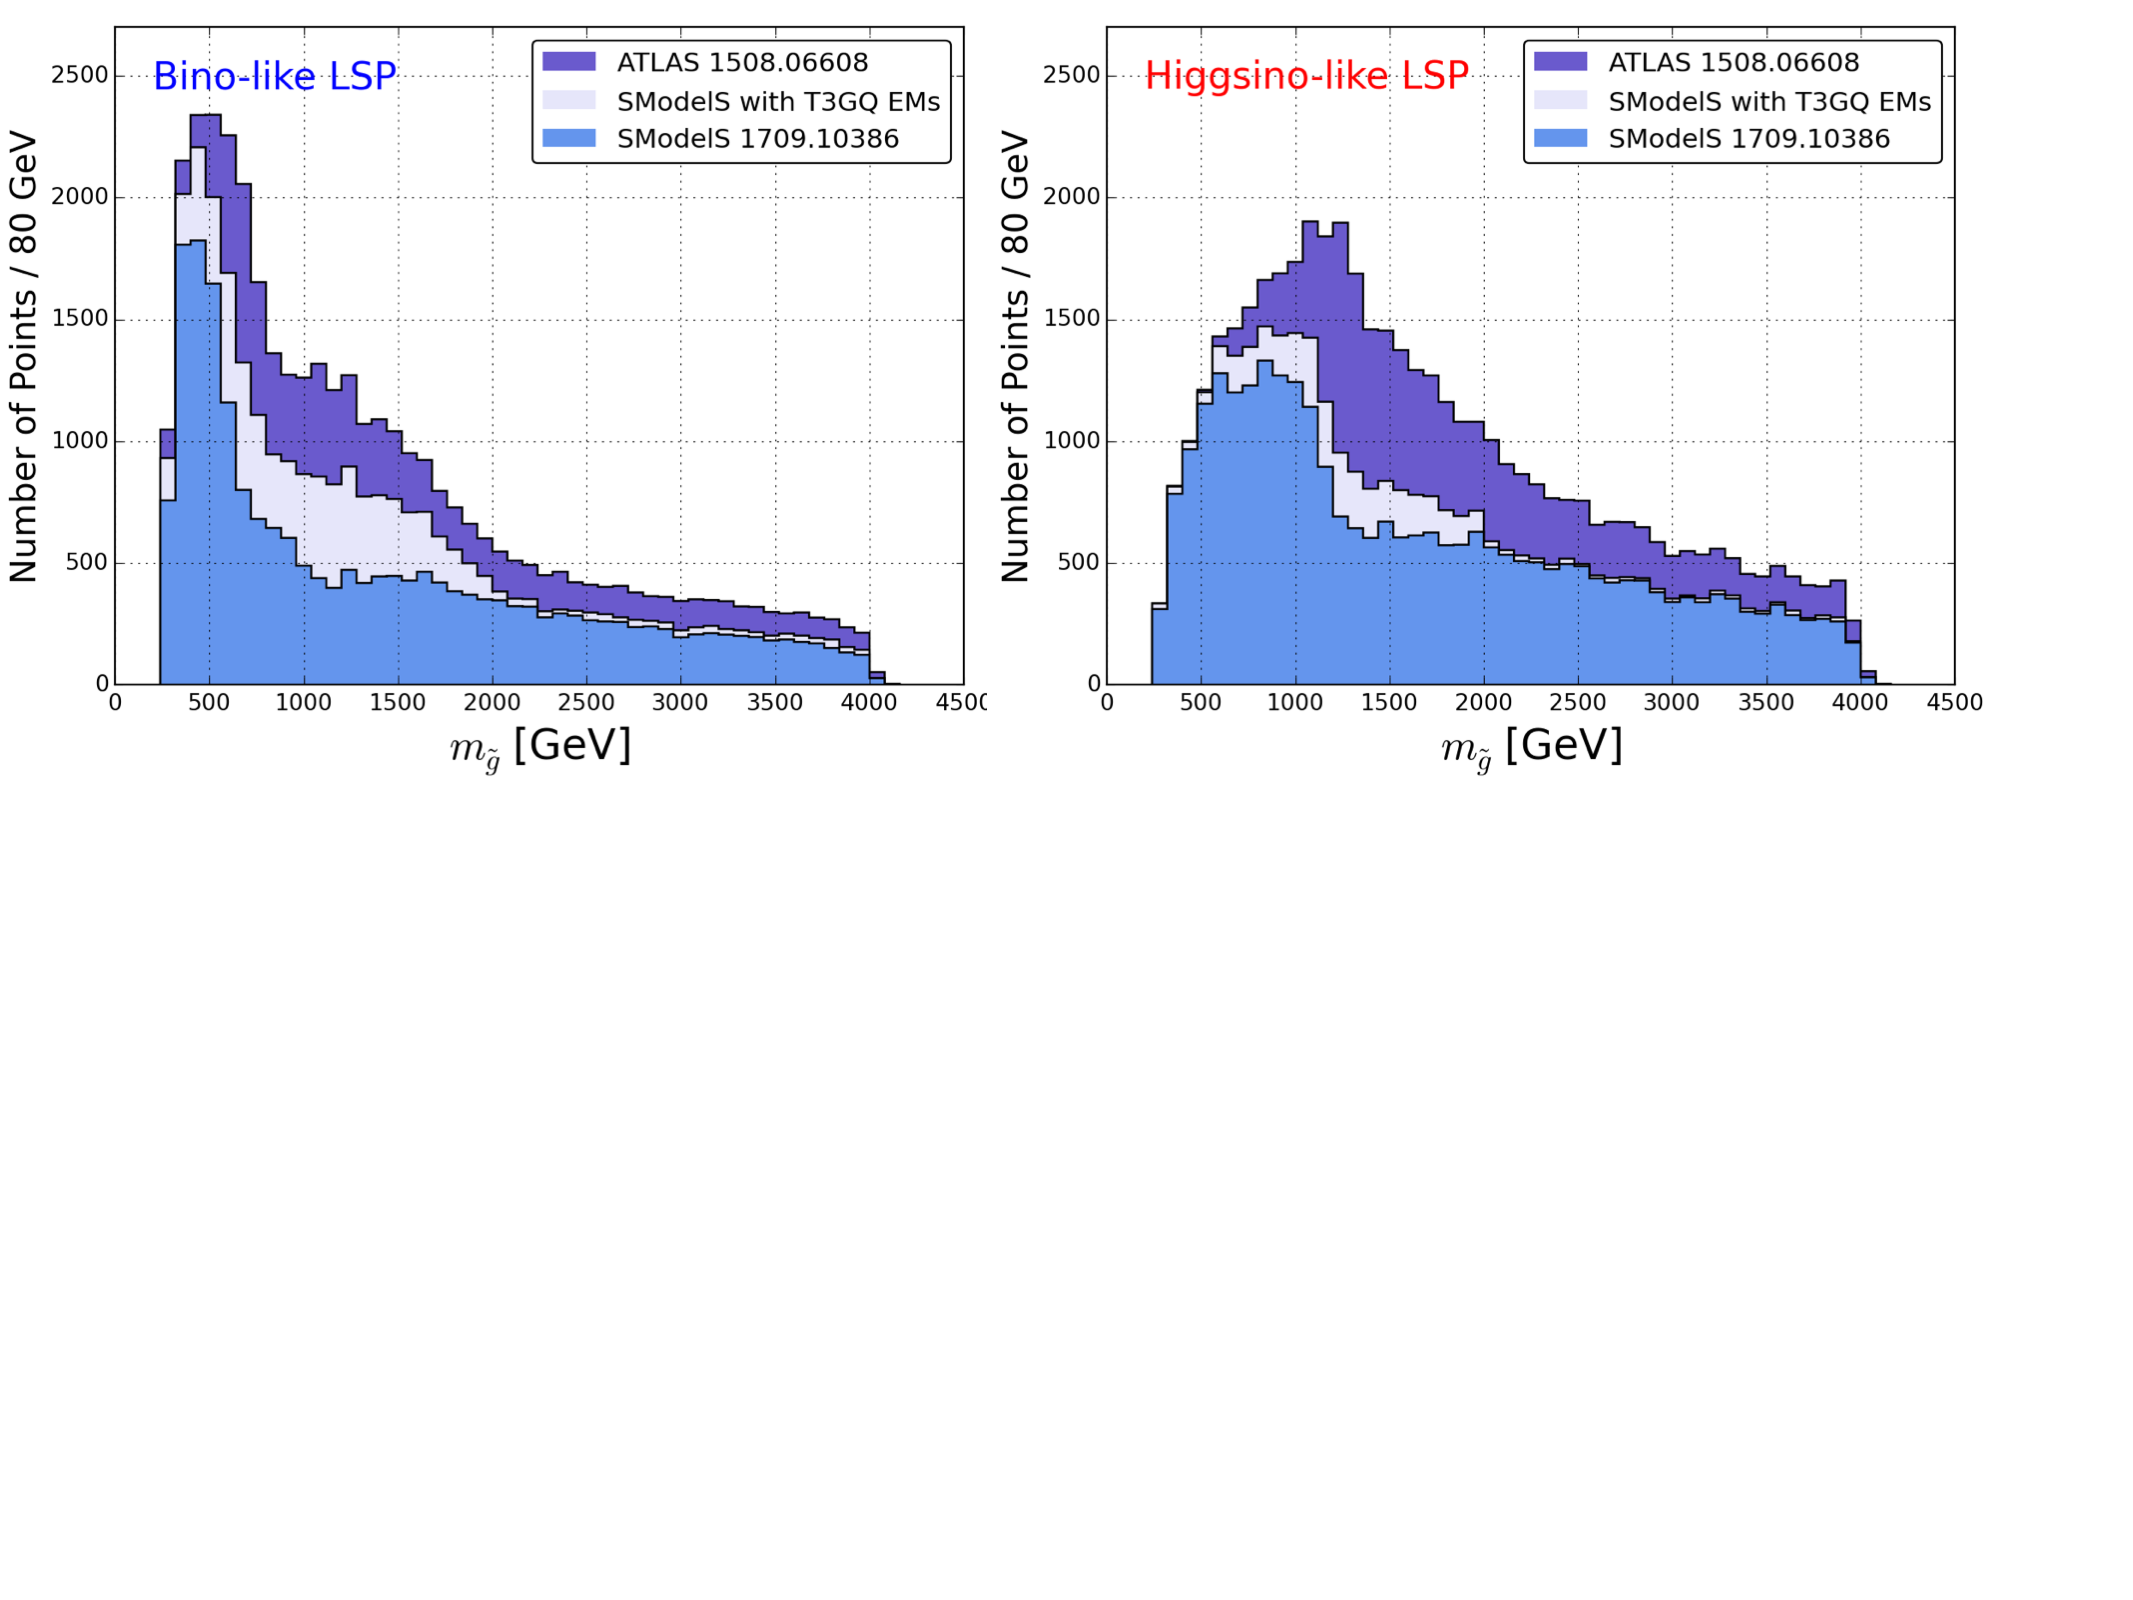
\includegraphics[width=1\textwidth]{PLOTS/New/New_Res.pdf}	
	\end{center}
	\caption{Distributions of the points excluded by ATLAS (purple), by \SMO~ with the inclusion of the newly home-grown maps (light blue), and by the previous work \cite{Ambrogi:2017lov} (slate blue), for the Bino(top) and Higgsino-like LSP (bottom).}
	\label{pmssm_new_exclusion_gluino}
\end{figure*}
We used the complete set of SMS results available for 8 TeV centre-of-mass energy of the release 1.1.1 of the database. These include official results in the form of upper limits and efficiency maps from the ATLAS and CMS collaborations, EMs results produced by the \texttt{FastLim} collaboration available at \cite{fastlim:web} and adapted to the \SMO~ infrastructure, and the set of EM results recast by \SMO~ collaboration. The complete description of the database of v1.1.1 can be consulted in \cite{Ambrogi:2017lov}). In addition we added the EM results specifically produced for this work described in Section \ref{EMprod}. Concretely, the additional EMs results in the updated database are:
\begin{itemize}
	\item ATLAS-SUSY-2013-02: \Ttwo~(which replaces the maps officially provided by ATLAS), \Tfive~and \TGQ~results; \
	\item CMS-SUS-13-012 \Ttwo~(which replaces the maps officially provided by CMS) and \TGQ~results.
\end{itemize}


The replacement of the \Ttwo results was done in order to cover smaller mass gaps, as described in Tab. \ref{TGQ_Planes}. The new EMs were made available with the database release 1.2.2. All the versions of \SMO~ databases can be consulted at \cite{databases}. For convenience, all the EMs results that will discussed when presenting the extension of the pMSSM-19 coverage are summarised in Tab.\ref{EMS}.


% 
\begin{wraptable}{r}{8cm}
	\begin{center}
		\renewcommand{\arraystretch}{1.1}
		\begin{tabular}{ c l c}  \toprule  \toprule 
			%\multicolumn{3}{c}{($M_1,M_2,M_3) = (1000,200,190)$} & \multicolumn{3}{c}{ \textbf{T3GQ}} & \multicolumn{3}{c}{ \textbf{T3QG}} \\  \toprule 
			\multicolumn{3}{c}{ATLAS-SUSY-2013-02 , CMS-SUS-13-012} \\ \toprule 
			SMS & Decay & Source \\ \toprule
			\textit{T1} &  $ p p \rightarrow \tilde g \tilde g, \tilde g \rightarrow q \bar q \tilde \chi_1 ^0 $ & Official \\
			\Ttwo & $  p p \rightarrow \tilde q \tilde q , \tilde q \rightarrow q \tilde \chi_1 ^0 $&  Recast\\
			\Tfive & $p p \rightarrow \tilde g \tilde g , \tilde g \rightarrow \tilde q q,  \tilde q \rightarrow q \tilde \chi_1 ^0 $& Recast  \\
			\TGQ & $ p p \rightarrow \tilde g \tilde q, \tilde g \rightarrow \tilde q q,  \tilde q \rightarrow q \tilde \chi_1 ^0 $ & Recast \\  
			\bottomrule \bottomrule                                             
		\end{tabular}
	\end{center}
	\caption{Summary of the EMs considered in the extension of the pMSSM-19 coverage.}
	\label{EMS}
\end{wraptable}
Note that several EMs results were recast for the CMS-SUS-13-012 analysis, and already employed for the coverage in the first study. finally, note that the focus of the rest of this work will be centred around the results provided by the ATLAS-SUSY-2013-02 EMs here described, mainly for two reasons. The first one is the availability of a direct comparison with the full recast performed by the ATLAS collaboration. The second one is that on average, the results from this analysis are more constraining with respect to the CMS counterpart. This is due to the specific design of the analysis: the signal regions in the ATLAS search are very inclusive hence the efficiency can capture a large portion of the SUSY signals within the same signal region. On the contrary, the CMS analysis defines 36 non-overlapping signal region, so that the SUSY signal is split into several bins (specifically the hadronic transverse energy, missing hadronic transverse energy and jet multiplicity bins). Since the combination of signal regions is not possible, only the best signal region is used to calculate the limits, that in general result weaker than the ATLAS search.
%

\section{Extending the pMSSM Coverage}\label{sec::impact}
In this Section we study the improvements in the pMSSM coverage provided by the additional EMs for the \textit{T3GQ} gluino-squark model, in combination with the \textit{T2} and \textit{T5} model. 
\\
%
\begin{table}[!h]
	\footnotesize
	\begin{center}
		\renewcommand{\arraystretch}{1.3}
		\begin{tabular}{l l c }  \toprule  \toprule 
			& \textbf{ATLAS} & \textbf{\SMO (EM+UL)} \\ \toprule \toprule 
			\textbf{Bino LSP} & &  \\
			& 38527 & 28765 (74 $\% $) \\ 
			\textbf{Higgsino LSP} & &   \\
			& 45345 & 32358 (71 $\% $) \\ \bottomrule   \bottomrule  
		\end{tabular}
	\end{center}
	\caption{\SMO~ constraints for the Bino and Higgsino-like LSP after the addition of the newly implemented EMs results for the models \textit{T2}, \textit{T5} and \textit{T3GQ}.}
	\label{Res_Tab_New}
\end{table}
%
Table \ref{Res_Tab_New} shows the new total exclusion of the pMSSM points, 21,151 and 28,669 points for the Bino and Higgsino-like case, allowing to cover the 74 and 71 $\%$ of the total points tested. With respect to the previous coverage detailed in \cite{Ambrogi:2017lov}, an improvement in the coverage of +19$\%$ and +8$\%$ respectively is obtained.
%
The major improvement appears in the Bino-like LSP case, as noticeable also in the gluino and squark mass coverage distributions in Fig. \ref{pmssm_new_exclusion_gluino}. Due to the choice of the parametrisation of the mass planes for the sample production, the bulk of the improvement is found for $m_{\tilde g}\leq$ 2 TeV. The extension of the EM to cover of the small mass gaps between the squarks and the LSP, as described in Tab. \ref{TGQ_Planes}, gives important contribution to the exclusion not only for large gluino masses, but also for intermediate to low mass values.
%
\subsection{Breakdown of the SMS Results}
\begin{figure*}
	\begin{center}
		\subfigure
		{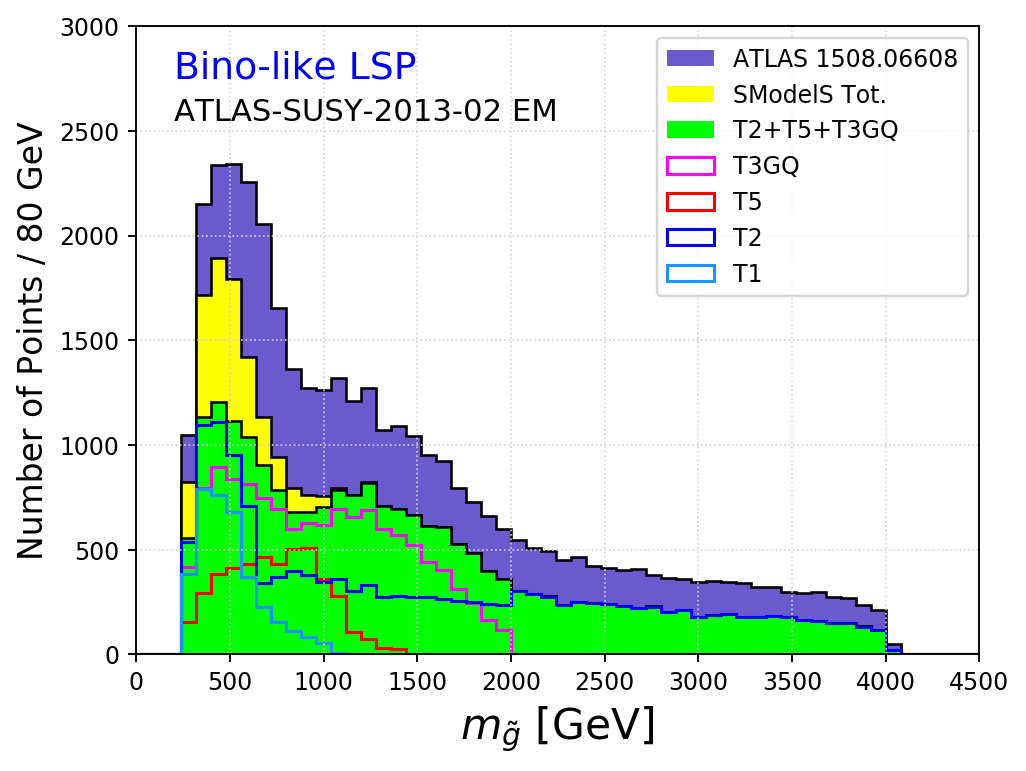
\includegraphics[width=0.49\textwidth]{PLOTS/Combination/Bino_Con.png}}
		\subfigure
		{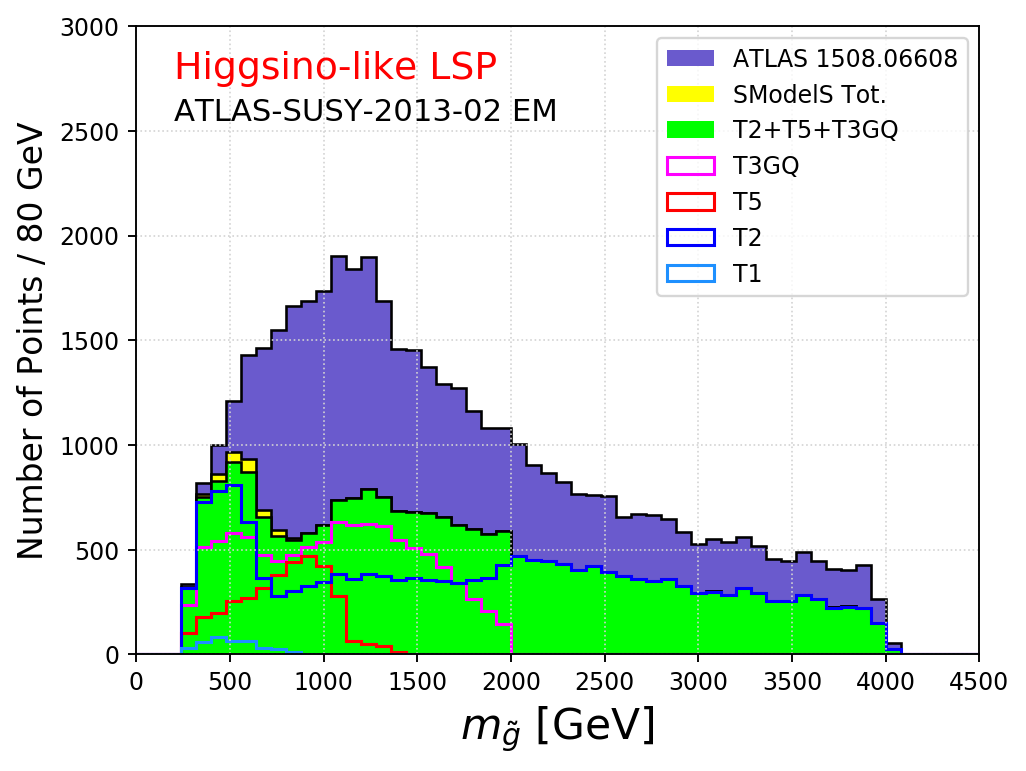
\includegraphics[width=0.49\textwidth]{PLOTS/Combination/Higgsino_Con.png}}
	\end{center}
	\caption{Contribution of the \textit{T1}, \textit{T2}, \textit{T5} and \textit{T3GQ} simplified model results and their combination for the analysis ATLAS-SUSY-2013-02, as a function of \MGLU.} 
	\label{sms-histo}
\end{figure*}
As detailed in Section \ref{sec::T3GQ}, the \textit{T2}, \textit{T5} and \textit{T3GQ} can be combined to reconstruct more comprehensively the signals from $\tilde g \tilde g$, $\tilde q \tilde q$ and $\tilde g \tilde q$ production channels. Here we wish to analyse how the newly excluded points benefit from such combination. We limit ourselves to consider only the analysis ATLAS-SUSY-2013-02, since similar conclusions can be obtained for the CMS-SUS-13-012 analysis. In addition we to the recast results, EMs for the \textit{T1} model 
\begin{equation}
p p \rightarrow \tilde g \tilde g , \tilde g \rightarrow q \bar q \tilde \chi_1 ^0 \ , 
\end{equation}
i.e. gluino decay to the LSP via off-shell light squarks, provided by the ATLAS collaboration, are used. The exclusions from each model and from the combination of the $T2+T5+T3GQ$ are drawn in Fig. \ref{sms-histo}. 
%
% HIGGSINO: the total number of points for gluino less that 1 TeV is  12058 6600 
% BINO: the total number of points for gluino less that 1 TeV is  17128 11675
%
%
Note that points can be excluded by more than one results, e.g. points with both light squarks and gluinos, with $m_{\tilde g} > m_{\tilde q}$, might be excluded by both the \textit{T2} and \textit{T5} results; for this reason, the histogram relative to each SMS cannot be stacked together. A major difference between the Bino and the Higgsino-like LSP case concerns the exclusion from the \textit{T1} results, which are significant in the former case, but almost irrelevant in the latter. The model is considered for completeness since such result is available. However, this signal cannot be in general combined with the other signatures of interest, since the \textit{T1} model arises most frequently from the decay of a gluino decaying to an off-shell squark, which is by construction a competing decay channel with respect to the \textit{T3GQ} model. Other SUSY configuration can still result in the \textit{T1} signature, for example the production of charginos and neutralinos decaying hadronically to off-shell vector bosons, but they are practically irrelevant due to the small $\sigma \times BR$.  
In Fig. \ref{fraction} the contribution of the model carrying the largest $r$ value (or partial weight) among the available \textit{T1}, \textit{T2}, \textit{T5} and \textit{T3GQ} is highlighted. For the majority of the points, this values amount to around half of the total weight, calculated using all the available EM results. Besides taking advantage of the availability of recasting tools, EM results are also extremely useful since they allow for the combination of signals, allowing for the reconstruction of full SUSY events. 
%
%
In the case of the \textit{T2}, \textit{T5} and \textit{T3GQ}, the squark-squark, gluino-gluino and gluino-squark productions and their consequent decays to the LSP.
%
%
\iffalse
\begin{verbatim}
ATLAS-02 Bino like excluded ONLY by that txname
Glu_T1_Only 3174
Glu_T2_Only 7221
Glu_T5_Only 191
Glu_TGQ_Only 3259
Glu_T2_T5_TGQ_Only 3320
Total points 24625
***
Glu_T1_Only 204
Glu_T2_Only 11180
Glu_T5_Only 160
Glu_TGQ_Only 2792
Glu_T2_T5_TGQ_Only 299
Total points 22823
\end{verbatim}
\fi
As stressed when introducing EMs, one of the advantages of using such kind of results is the possibility to combine the different SUSY signals that map onto the decomposed SMS. In Table \ref{breakdown_number} the number of points that can be excluded only by the specific model listed is provided. This means that, for example, the \Tone model results can exclude 3,175 model points of the Bino-like LSP dataset i.w. the individual \RVALUE for this results exceeds unity. On the opposite, the \RVALUE of the sum of remaining results is insufficient to exclude the point. We see that, in this sense, the most powerful results is certainly the \Ttwo~; at the same time, around 3.000 points can only be excluded by the sum of (\Ttwo~ +\Tfive~ +\TGQ~) results.
\begin{table}[!h]
	\footnotesize
	\begin{center}
		\renewcommand{\arraystretch}{1.3}
		\begin{tabular}{ l c c }  \toprule \toprule
			\textbf{SMS} & \textbf{Bino} & \textbf{Higgsino} \\  \toprule
			\Tone~:$p p \rightarrow \tilde g \tilde g , \tilde g \rightarrow q \bar q \tilde \chi_1 ^0$ & 3174 & 204   \\
			\Ttwo~:$p p \rightarrow \tilde q \tilde q , \tilde q \rightarrow q \tilde \chi_1 ^0$ & 7221 & 11180 \\
			\Tfive~:$p p \rightarrow \tilde g \tilde g , \tilde g \rightarrow q \tilde q , \tilde q  \rightarrow q \chi_1 ^0$ & 191 & 160  \\
			\TGQ~:$p p \rightarrow \tilde q \tilde g , \tilde g \rightarrow q \tilde q , \tilde q  \rightarrow q \chi_1 ^0$ & 3259 & 2792  \\
			\Ttwo~ +\Tfive~ +\TGQ~ & 3320 & 299 \\
			\bottomrule \bottomrule 
			%\multicolumn{3}{l}{\Ttwo: $p p \rightarrow \tilde q \tilde q$} \\
		\end{tabular}
	\end{center}
	\caption{Number of points that can be excluded only by including each individual result for \Tone~,\Ttwo,\Tfive,\TGQ, or their combination. See the text for details.}
	\label{breakdown_number} 
\end{table}
Finally, in Fig. \ref{rvalues-bino} the distribution for the r-values for the \textit{T2}, \textit{T5}, \textit{T3GQ} models and their combination is shown, for the Bino and Higgsino-like LSP cases respectively. The contribution from the \textit{T1} model is not considered. Note that the plots are projected onto the $(m_{\tilde g}, min(m_{\tilde q}))$ mass plane. This highlights the contribution from the two alternative mass hierarchies $m_{\tilde g} > min(m_{\tilde q})$ or $min(m_{\tilde q}) > m_{\tilde g} $, clearly indicated by the points distributed around the diagonal of the plots.  {\color{blue} fill the space .}

\begin{figure}[!h]
	\begin{center}
		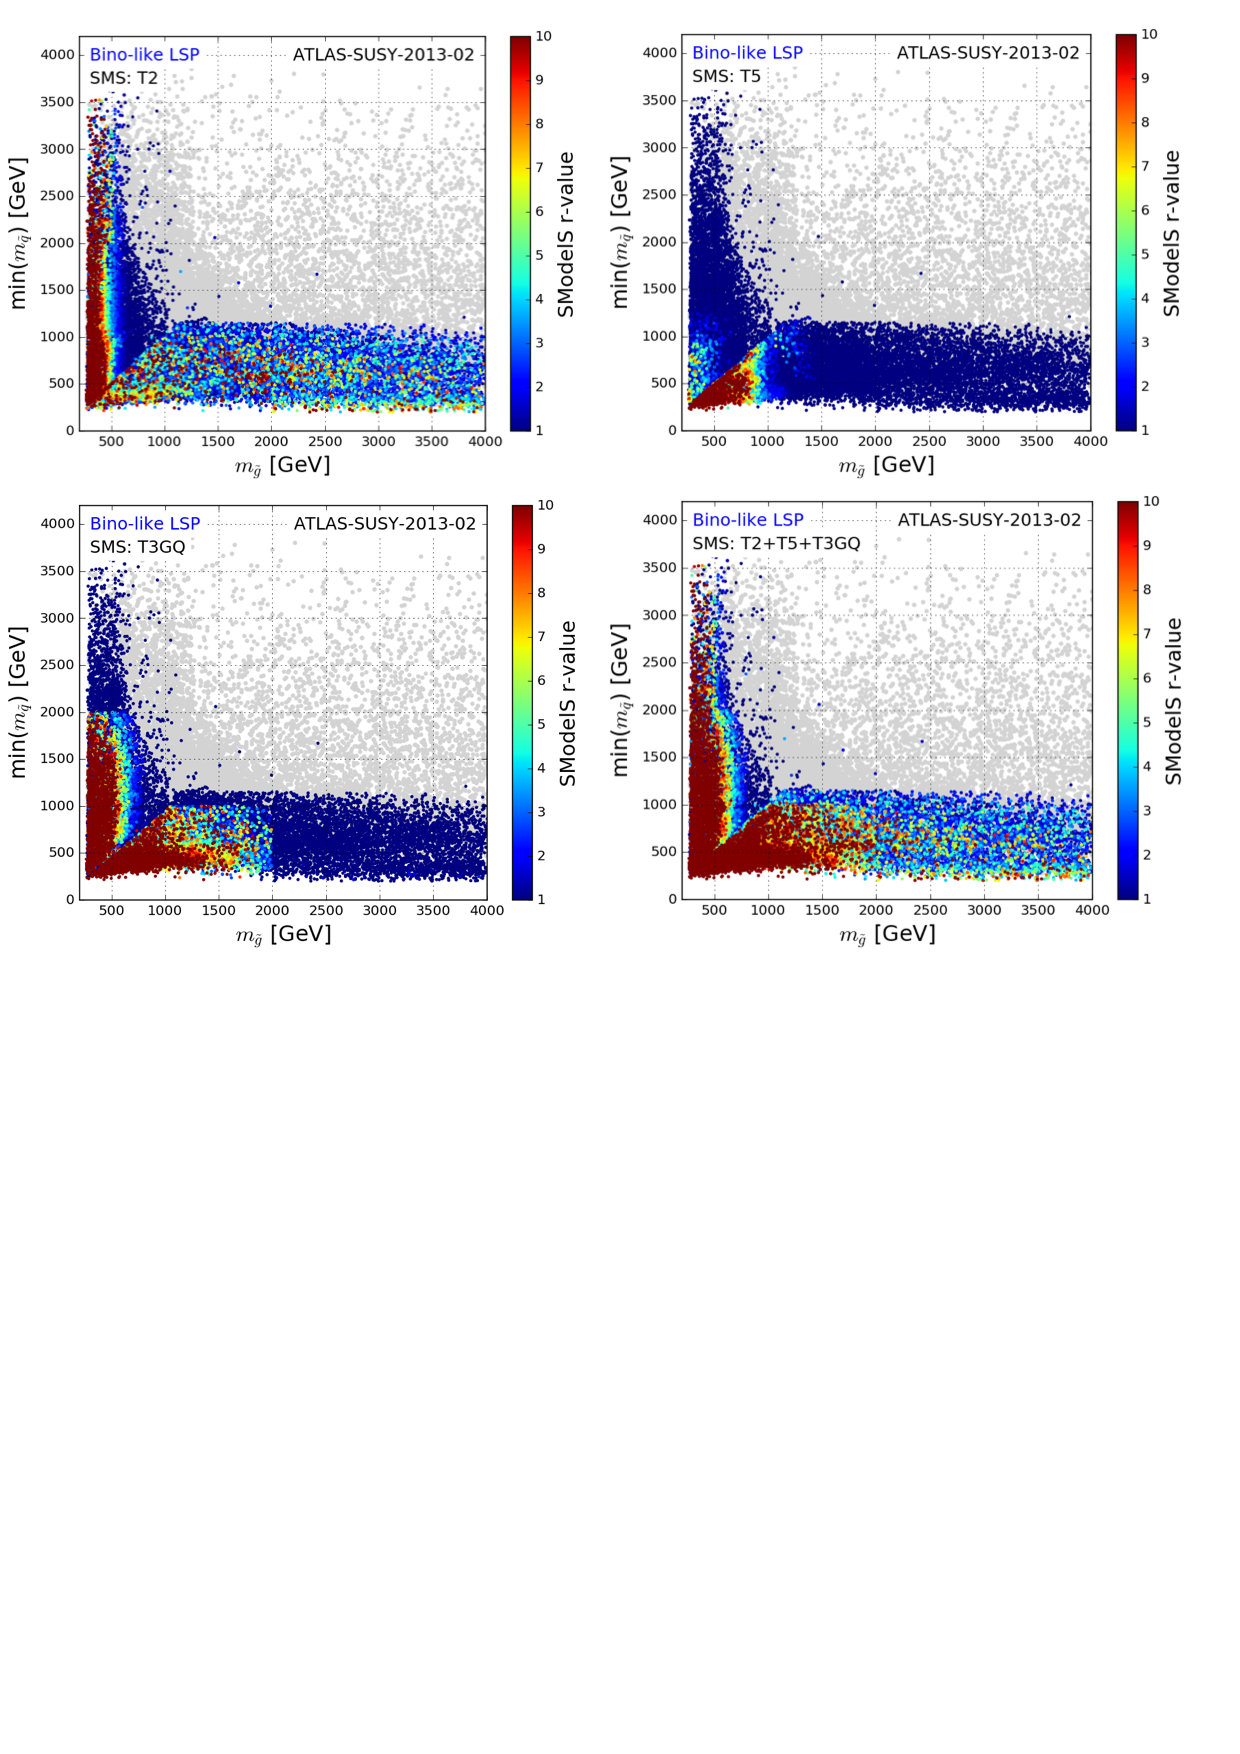
\includegraphics[width=1\textwidth]{PLOTS/App/Bino_Combo.pdf}
	\end{center}
	\vspace{0.2pt}
	\caption{Distributions of the \RVALUE for \textit{T2}, \textit{T5}, \textit{T3GQ} and their combination for the points excluded by the ATLAS-SUSY-2013-02 results (Bino-like LSP dataset). Grey points have a total $r$ value $\leq$ 1. A large portion of points excluded bz \Ttwo~ lies in the $m_{\tilde g}<$500 GeV mass, due to the gluino loop decay $\tilde g \rightarrow g \tilde \chi _1 ^0$. A similar argument holds for the \Tfive~ model, in the region where the result constrains the $\tilde q \rightarrow q \tilde g, \tilde g \rightarrow  g \tilde \chi _1 ^0$ decay. The \TGQ~model results can efficiently constrain the two alternative mass hierarchies $m_{\tilde g}>m_{min(\tilde q)}$ or $m_{min(\tilde q)}>m_{\tilde g }$. In particular it shows that the EMs should be extended to cover \MGLU~masses larger than the 2 TeV values.}
	\label{rvalues-bino}
\end{figure}
%
%
\iffalse
\begin{figure}[!]
	\begin{center}
		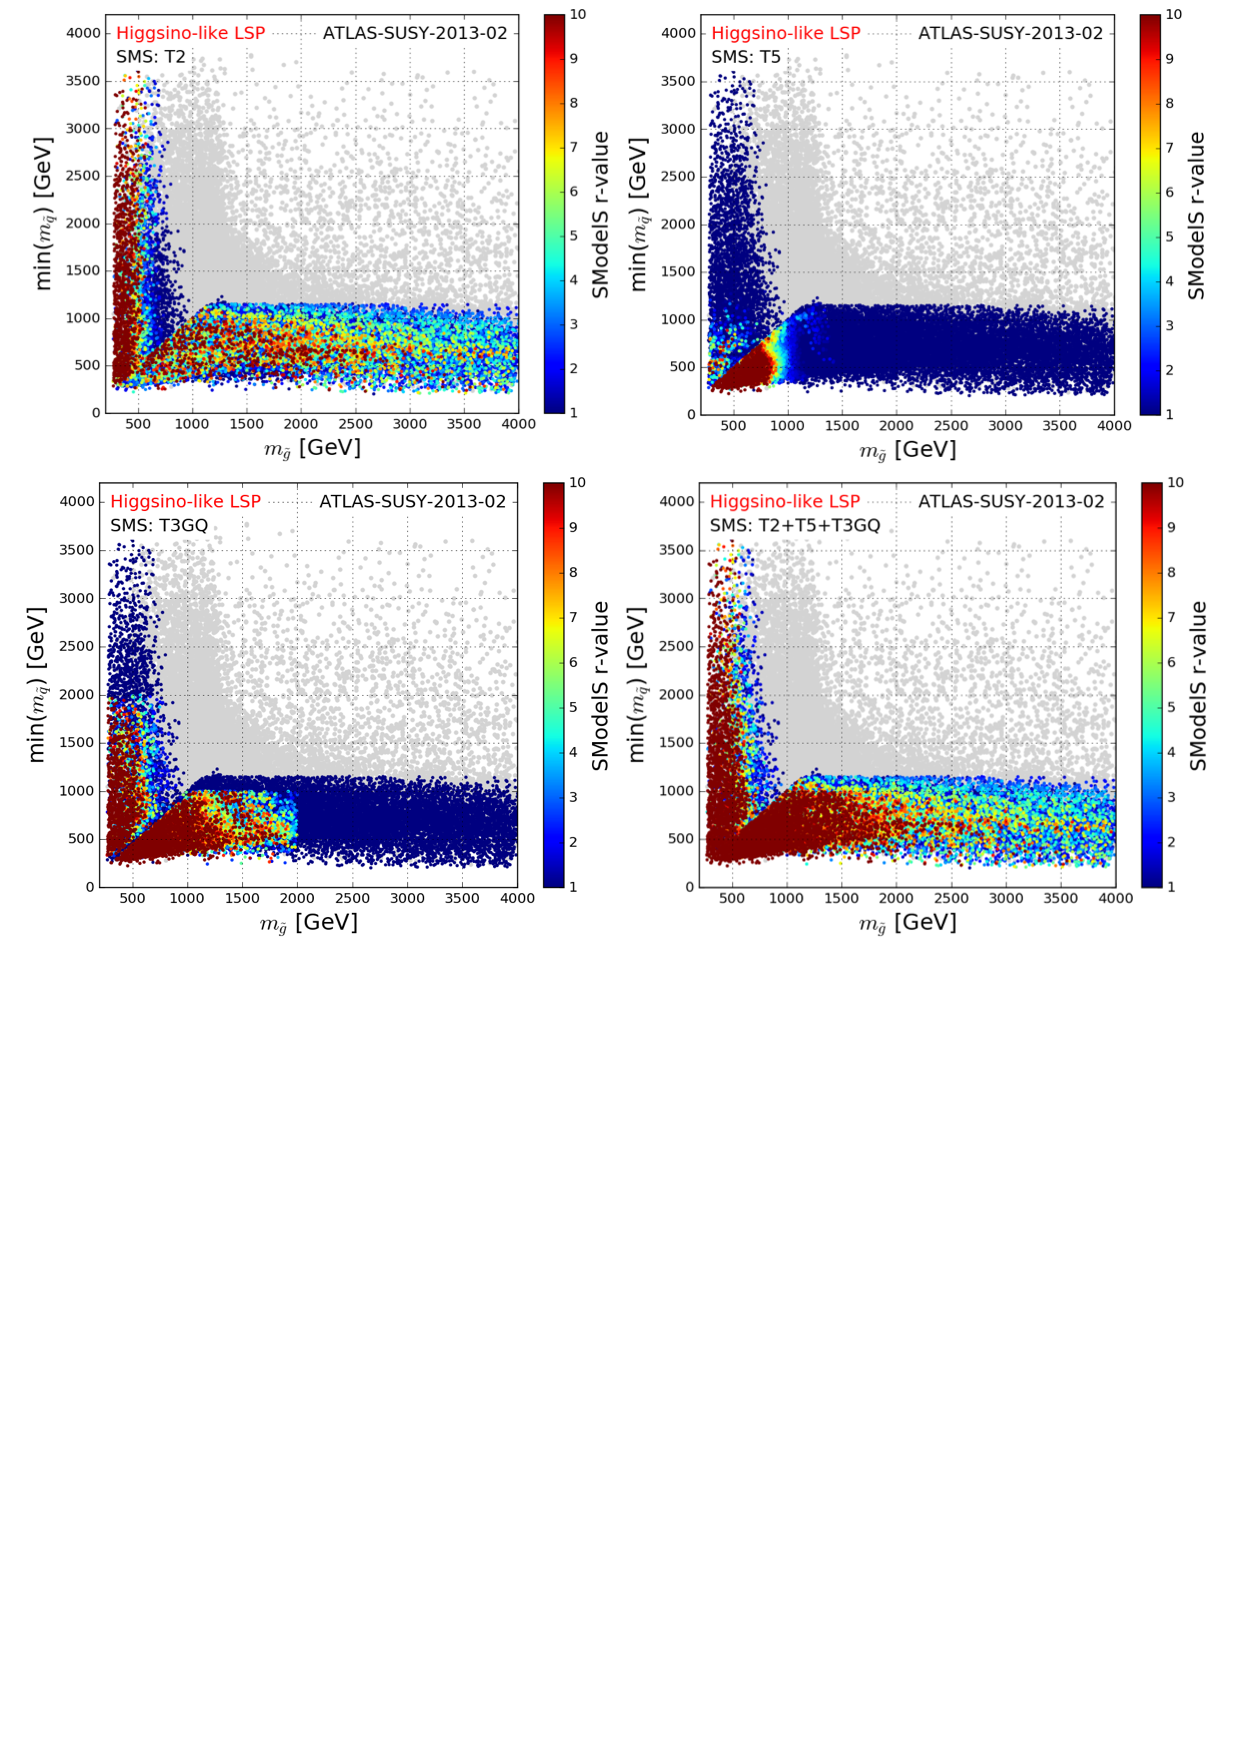
\includegraphics[width=1\textwidth]{PLOTS/App/Higgsino_Combo.pdf}
	\end{center}
	\caption{Same as Fig. \ref{rvalues-bino} for the Higgsino-like LSP dataset.} 
	\label{rvalues-higgsino}
\end{figure}
\fi
%
\subsection{Estimation of the Uncertainties}\label{estimation}
\begin{figure}[!h]
	\begin{center}
		\subfigure
		{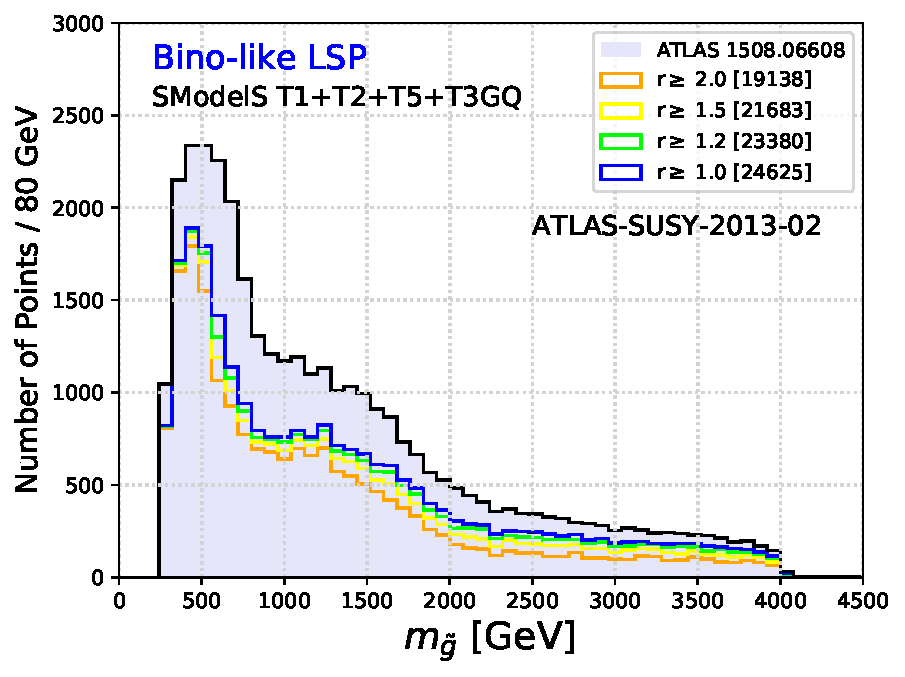
\includegraphics[width=0.49\textwidth]{PLOTS/Combination/Bino_TOT_GLU_Histo_rValue.pdf}}
		\subfigure
		{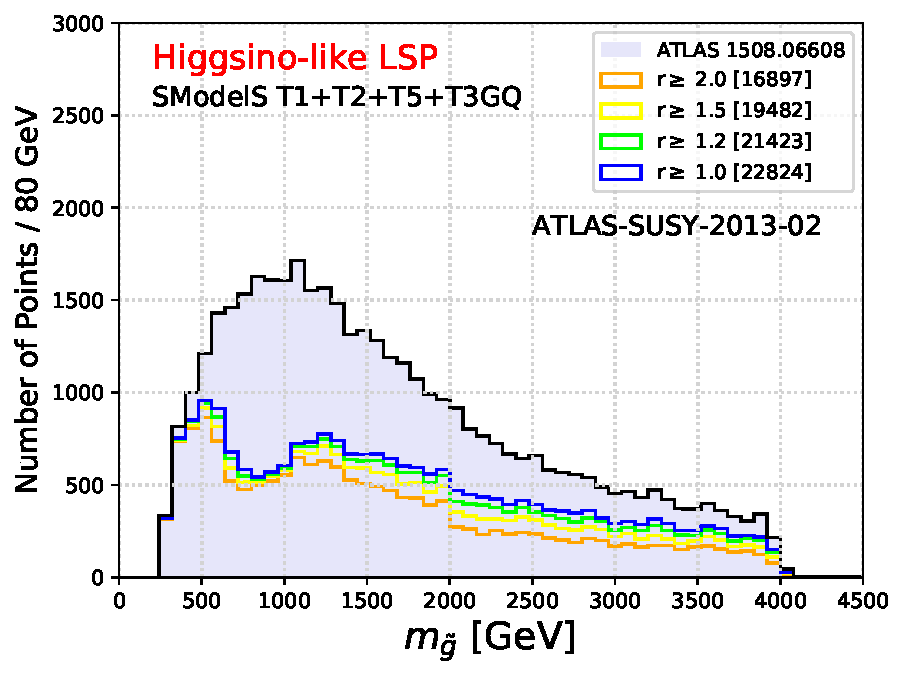
\includegraphics[width=0.49\textwidth]{PLOTS/Combination/Higgsino_TOT_GLU_Histo_rValue.pdf}}
	\end{center}
	\caption{Distribution of the excluded points, as a function of \MGLU, for different requirements of \RVALUE$>1.0,1.2,1.5,2.0$. Only the EM results for the analysis ATLAS-SUSY-2013-03 are used, for the SMS T1 (official results form ATLAS) and \Ttwo,\Tfive,\TGQ (homegrown \SMO~ results). On top, the total number of points excluded by the official ATLAS study only the aforementioned analysis is shown. } 
	\label{unc}
\end{figure}
In this section we provide a rough yet qualitative estimation of the uncertainties of the whole procedure. These are very challenging to estimate reliably due to the complexity of the procedure itself, which involves at first the production of the Monte Carlo events for the generation of the event files, then the analyses recast. The validation documents provided with the analyses recasting code is a valid proof that the choice of the simulation parameters allows to reproduce well the analyses efficiency. While the generation of a sufficient amount of events keeps the statistics uncertainty under reasonable control, systematic effects are not taken into accounts. Last but not least, the entire assumptions at the basis of the simplified model spectra idea inevitably introduces approximations, due to neglecting the production mechanisms of the SUSY particles considered (since the events are produced with decoupled spectra ) and any kinematics effects due to the quantum numbers of the particles. All these aspects add up together and cannot be easily quantified. As formulated in the definition of \SMO~ \RVALUE~in Eq. \ref{rvalue}, a model point is considered excluded if the \RVALUE exceeds unity. Tightening this condition by requiring that the theory predictions exceeds higher value can mimic the inclusion of uncertainties on the theory level (e.g. on the reference cross section calculation, on the recasting procedure and/or on the SMS assumptions). 
In Fig. \ref{unc} the distribution of the excluded points, as a function of \MGLU, is plotted for different \RVALUE~requirements of $r\ value >1$ (standard exclusion criterion used throughout the paper), and $r\ value >1.2 , 1.5,2.0$, corresponding to a decrease in the theory predictions of $20\%,50\%,100\%$. These higher values result in more conservative exclusion. The total number of points excluded considering each separated value is reported in the legend. It is comforting to note that even for the pessimistic case of the largest uncertainty, the number of points does not differ for more than $25\%$ with respect to the standard criterion. There is also no sign of higher impact which depends on \MGLU, so any systematic effect dependent on this mass parameter should be improbable. 
%It is of interest to quantify how much an uncertainty from the theory side can affect the overall exclusion in terms of number of points excluded. This is visualised in Fig. \ref{pmssm_new_rvalue}. The distributions show the total number of points excluded by the analysis ATLAS-SUSY-2013-02 for different requirements on of r $\geq$ (1.0, 1.2, 1.5, 2.0). This is equivalent to the inclusion of uncertainties by re-scaling the $( \sigma \times \epsilon )$, or \SMO~ theory predictions, by (0, 20, 50, 100)$\%$. I remind that all the previous plots showing excluded points assumed $r>$1 as standard exclusion criterion. In Tab. \ref{tab::rvalues} the numbers of excluded points are explicitly reported. For $r>$1.2 the difference is around 5(6)$\%$ and 12(15)$\%$ for the Bino(Higgsino)-like LSP case. Note finally that the theory cross section used by \SMO~ is not exactly the theory cross section used by the ATLAS collaboration, but was calculated by \SMO~ as described in Sec. \ref{pMSSM_setup}. 
%
We finally note than a similar methodology was employed by the ATLAS collaboration to determine the exclusion of the model points. In particular, the uncertainty on the theory cross section calculation was estimated up to $100\%$, but unfortunately such values are not available.
%
%\begin{figure*}
%\begin{center}
%\subfigure
%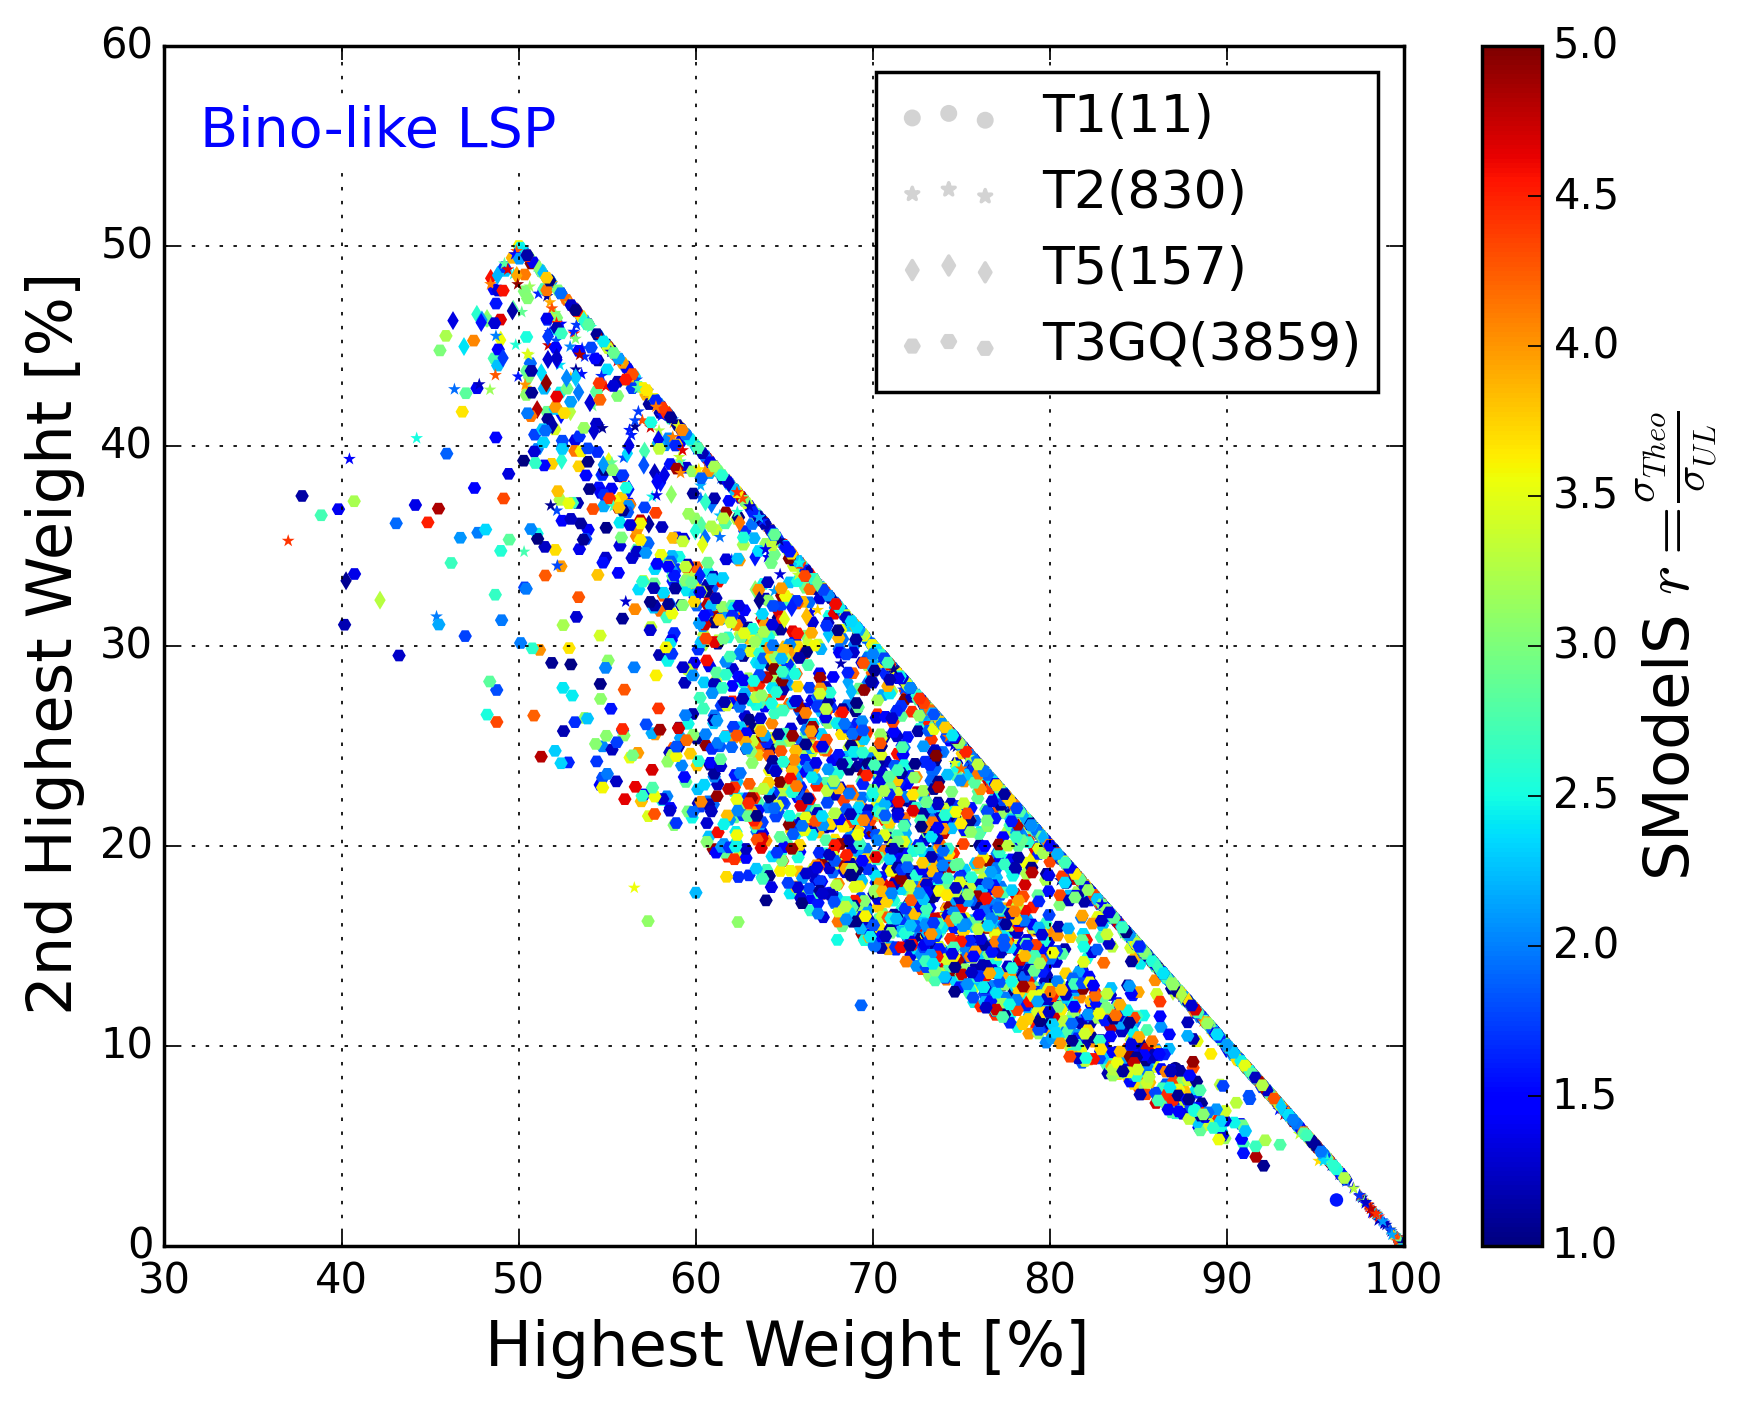
\includegraphics[width=0.49\textwidth]{PLOTS/Weights/Weight_Fraction_r5BINO.png}
%\subfigure
%{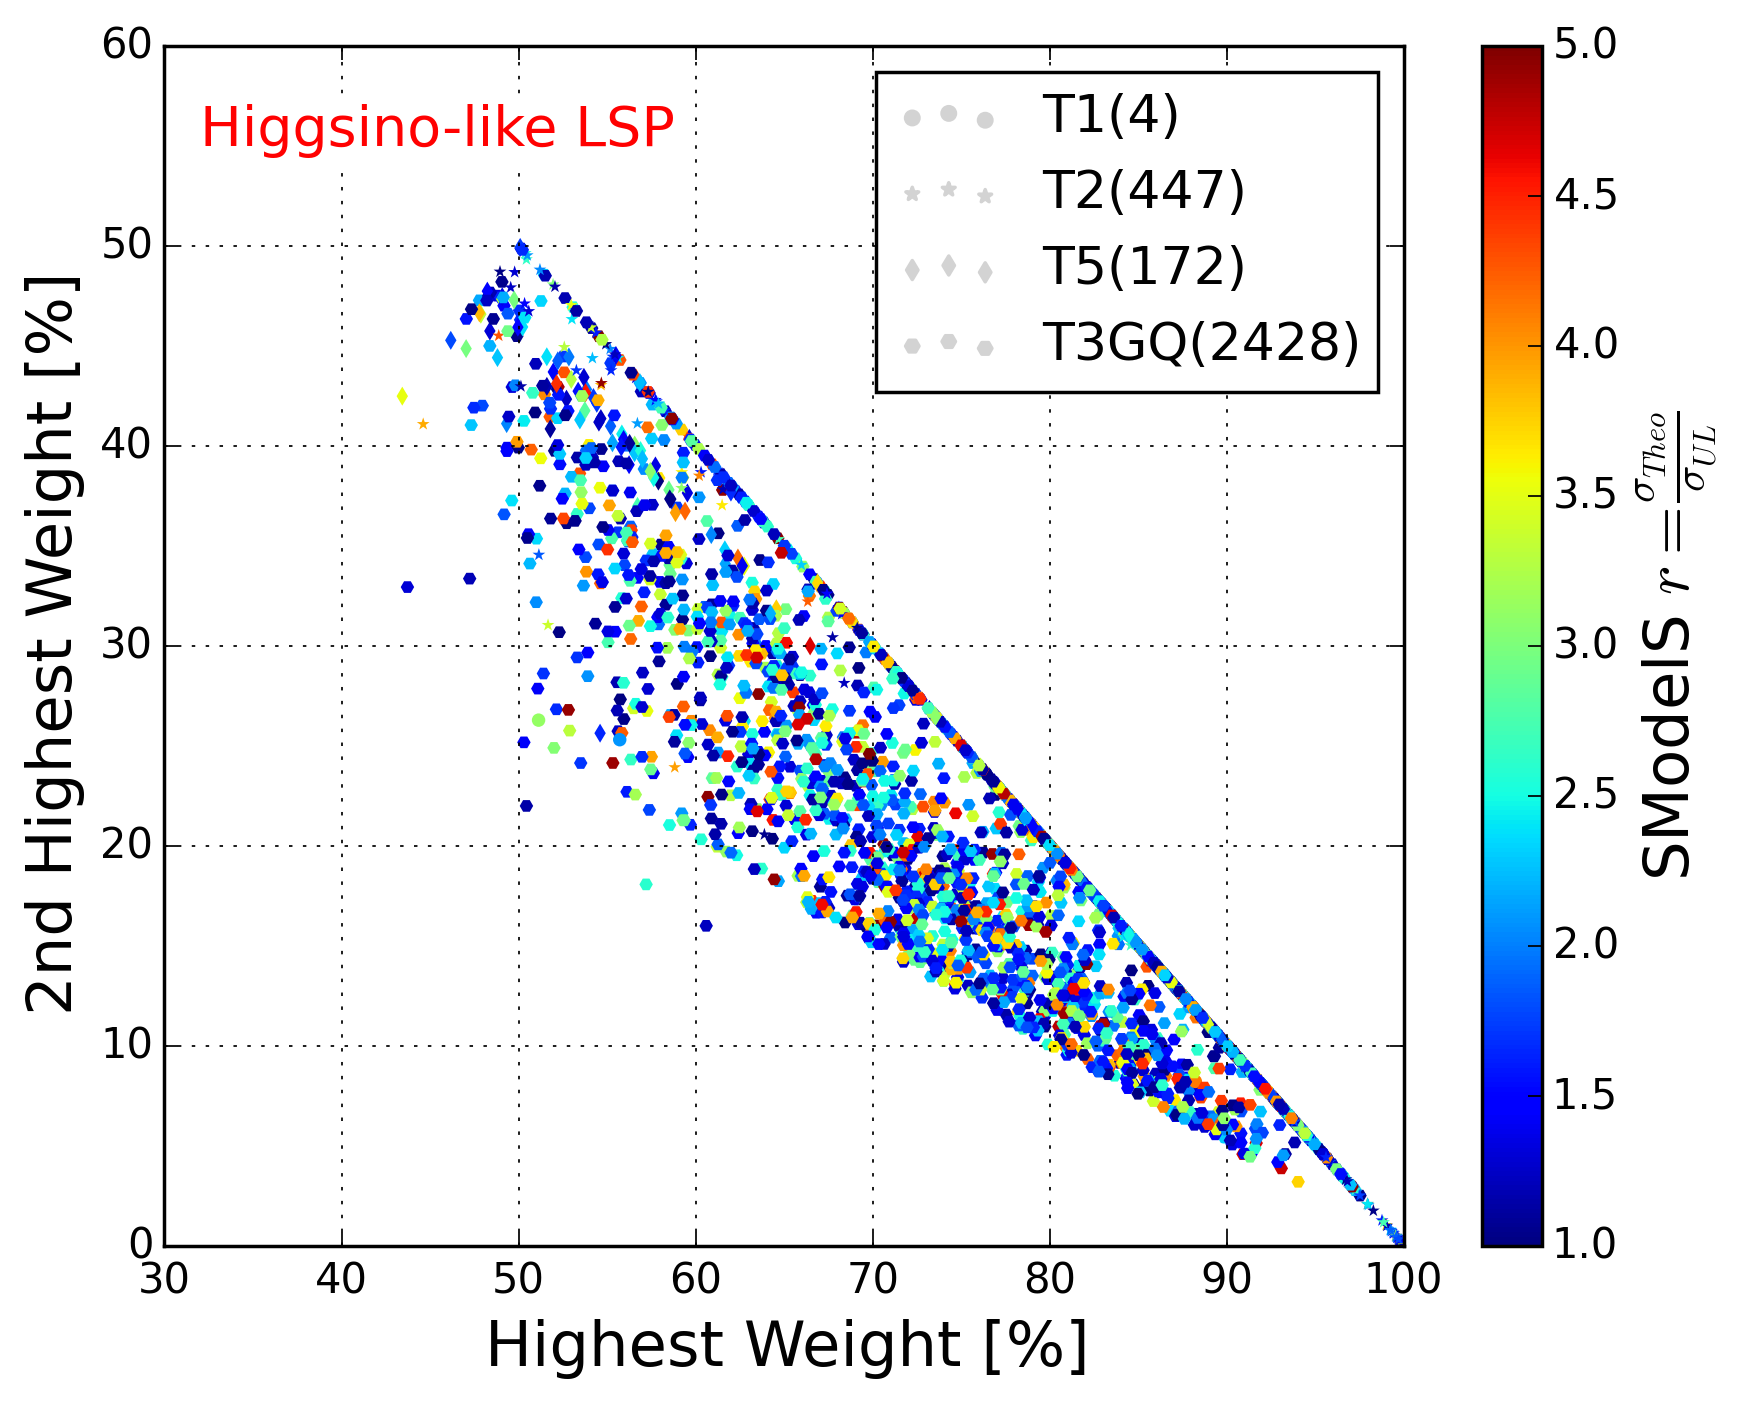
\includegraphics[width=0.49\textwidth]{PLOTS/Weights/Weight_Fraction_r5HIGGSINO.png}}
%\end{center}
%\caption{$\%$ contribution to the total weight of the highest (x-axis) and second highest (y-axis) topology, for the Bino-like (left) and Higgsino-like LSP (right). The topology leading the largest contribution is indicated with different marks. The color maps report the total rvalue for the analysis ATLAS-SUSY-2013-02; only points with rvalue<5 are shown. 
%{\color{blue} add ATLAS-02 label} }
%\label{rValues}
%\end{figure*}
%
%\subsection{Missing Topologies}
%Finally, it is interesting to have a look at the most important missing topologies. 
%\begin{figure}[!]
%\begin{center}
%\subfigure
%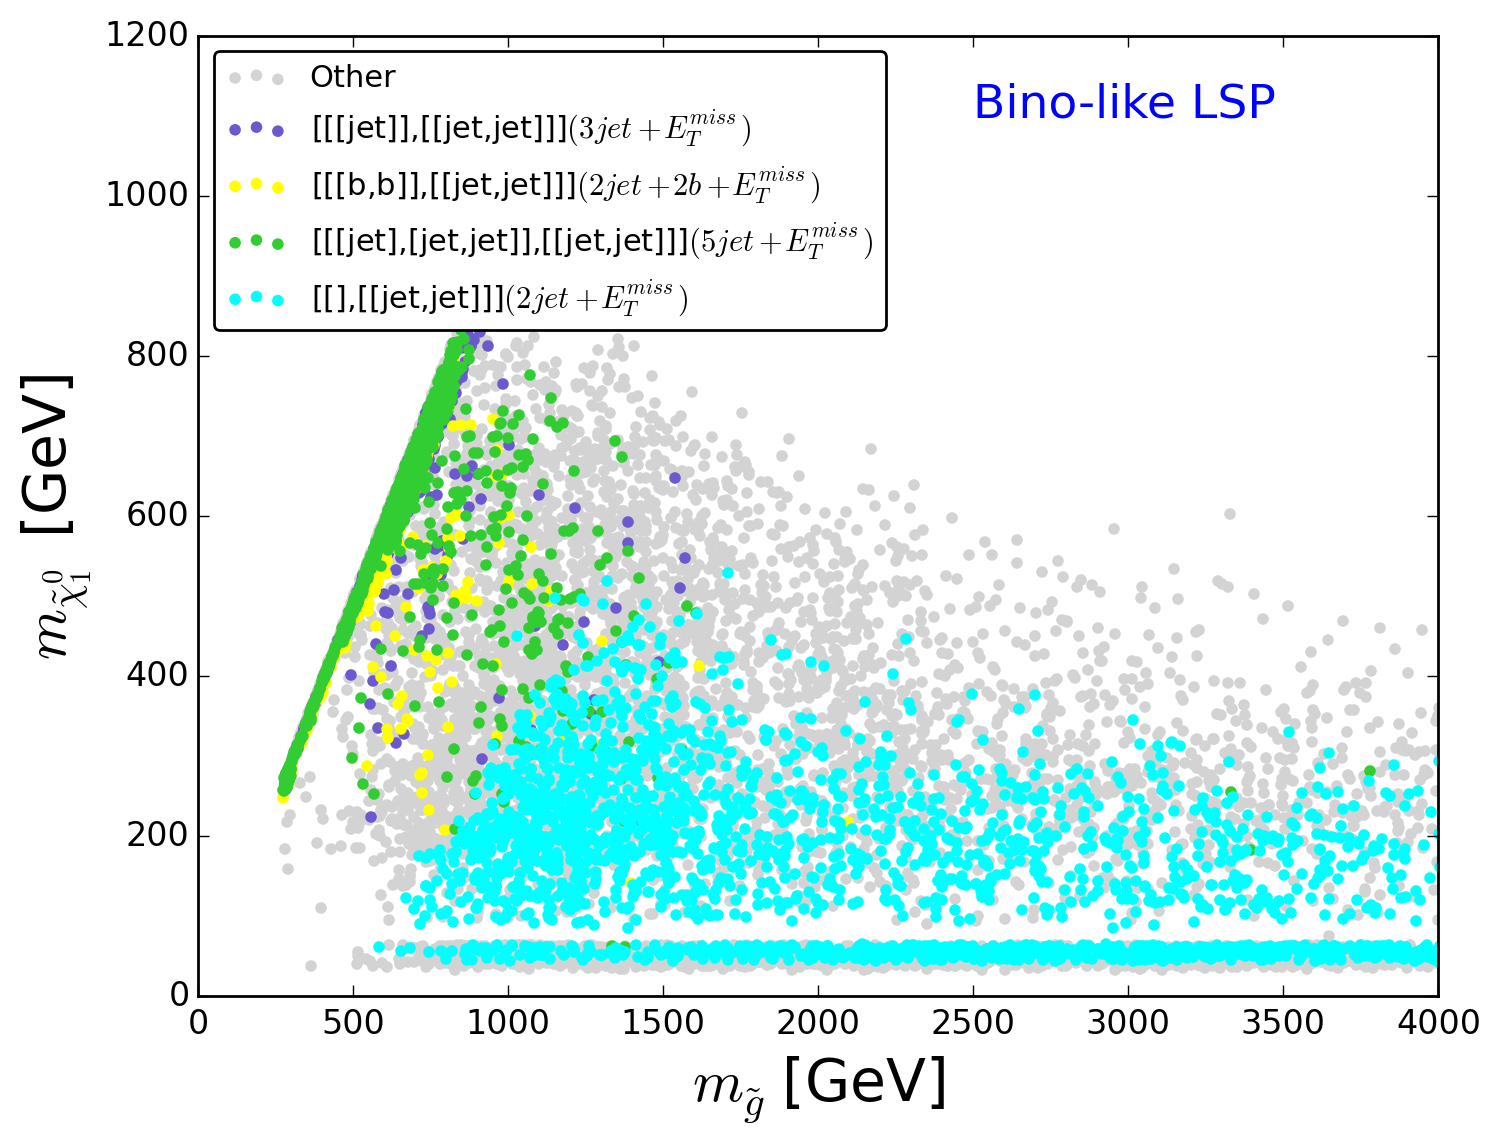
\includegraphics[width=0.49\textwidth]{PLOTS/Missing/BINO_Missing_GluNeu.png}
%\subfigure
%{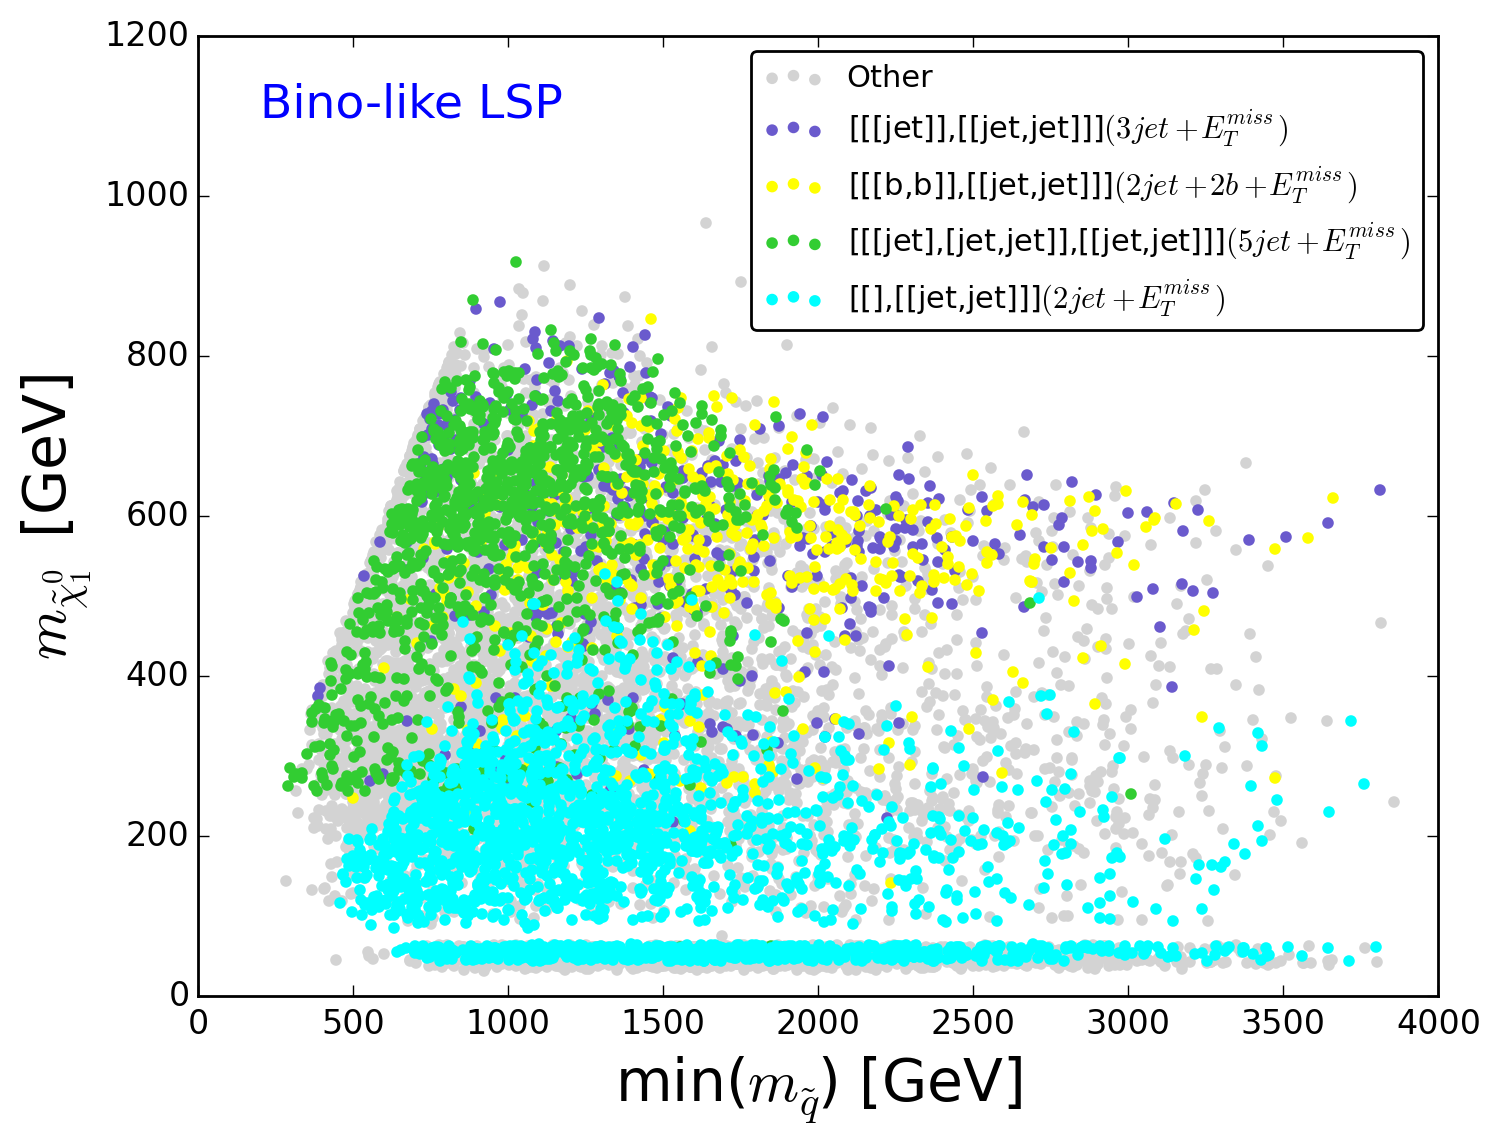
\includegraphics[width=0.49\textwidth]{PLOTS/Missing/BINO_Missing_SqNeu.png}}
%\subfigure
%{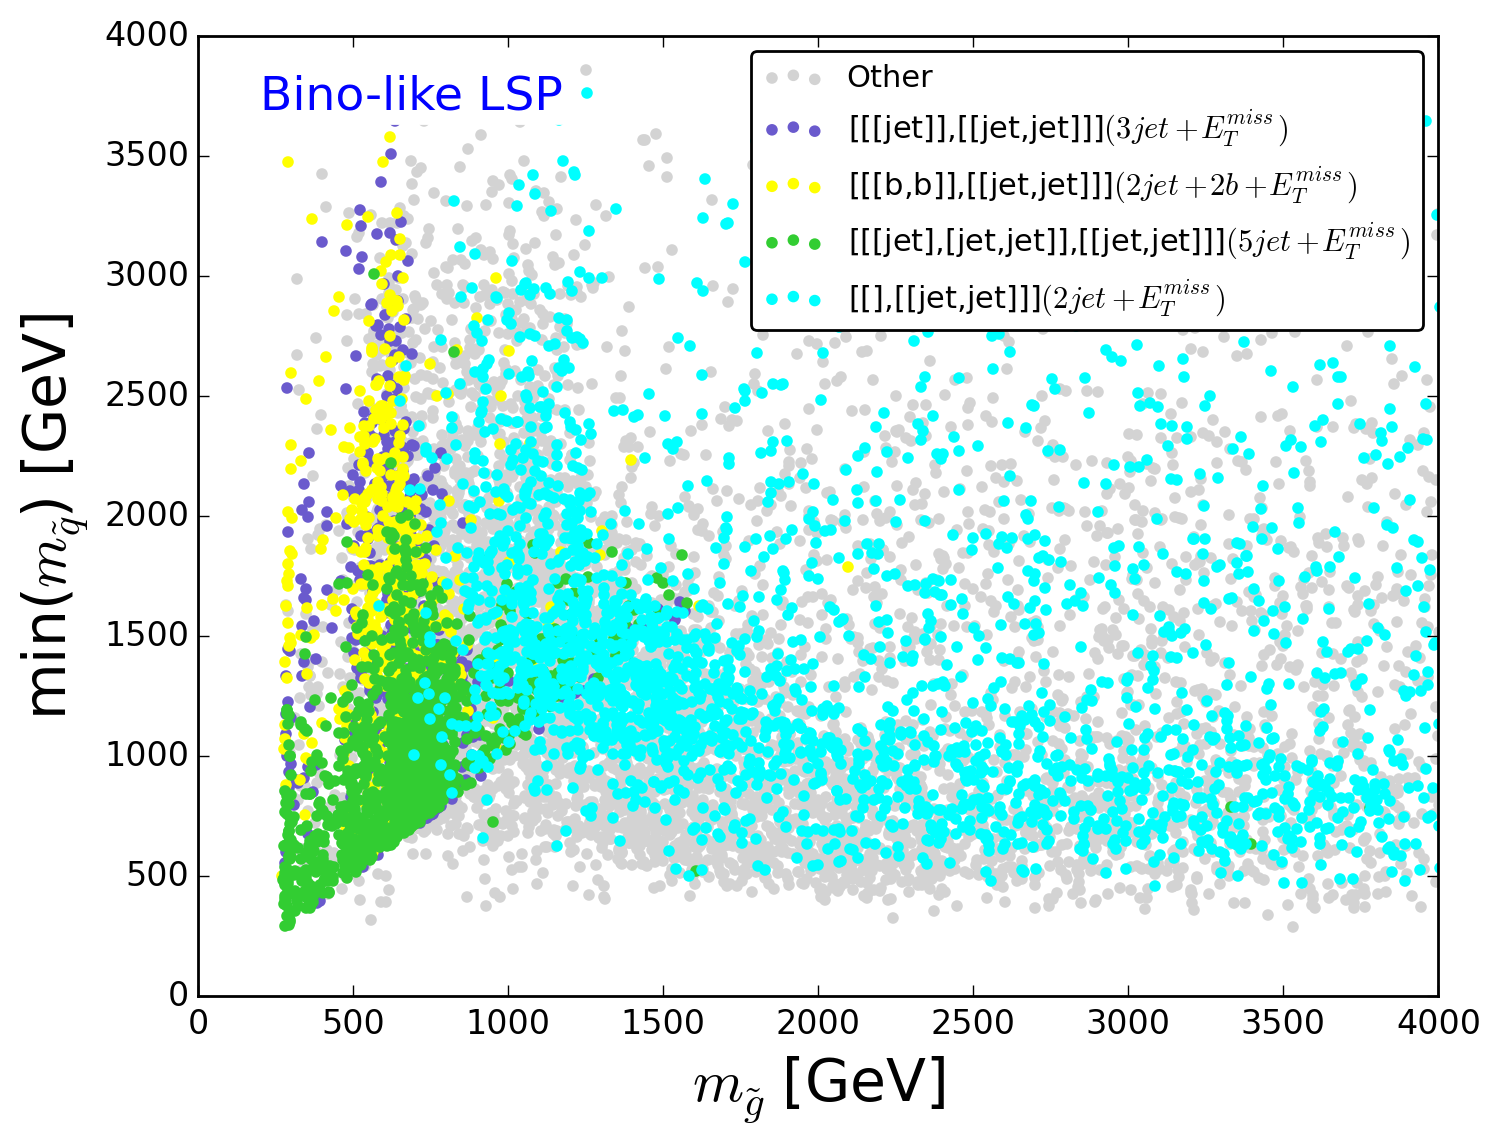
\includegraphics[width=0.49\textwidth]{PLOTS/Missing/BINO_Missing_GluSq.png}}
%\subfigure
%{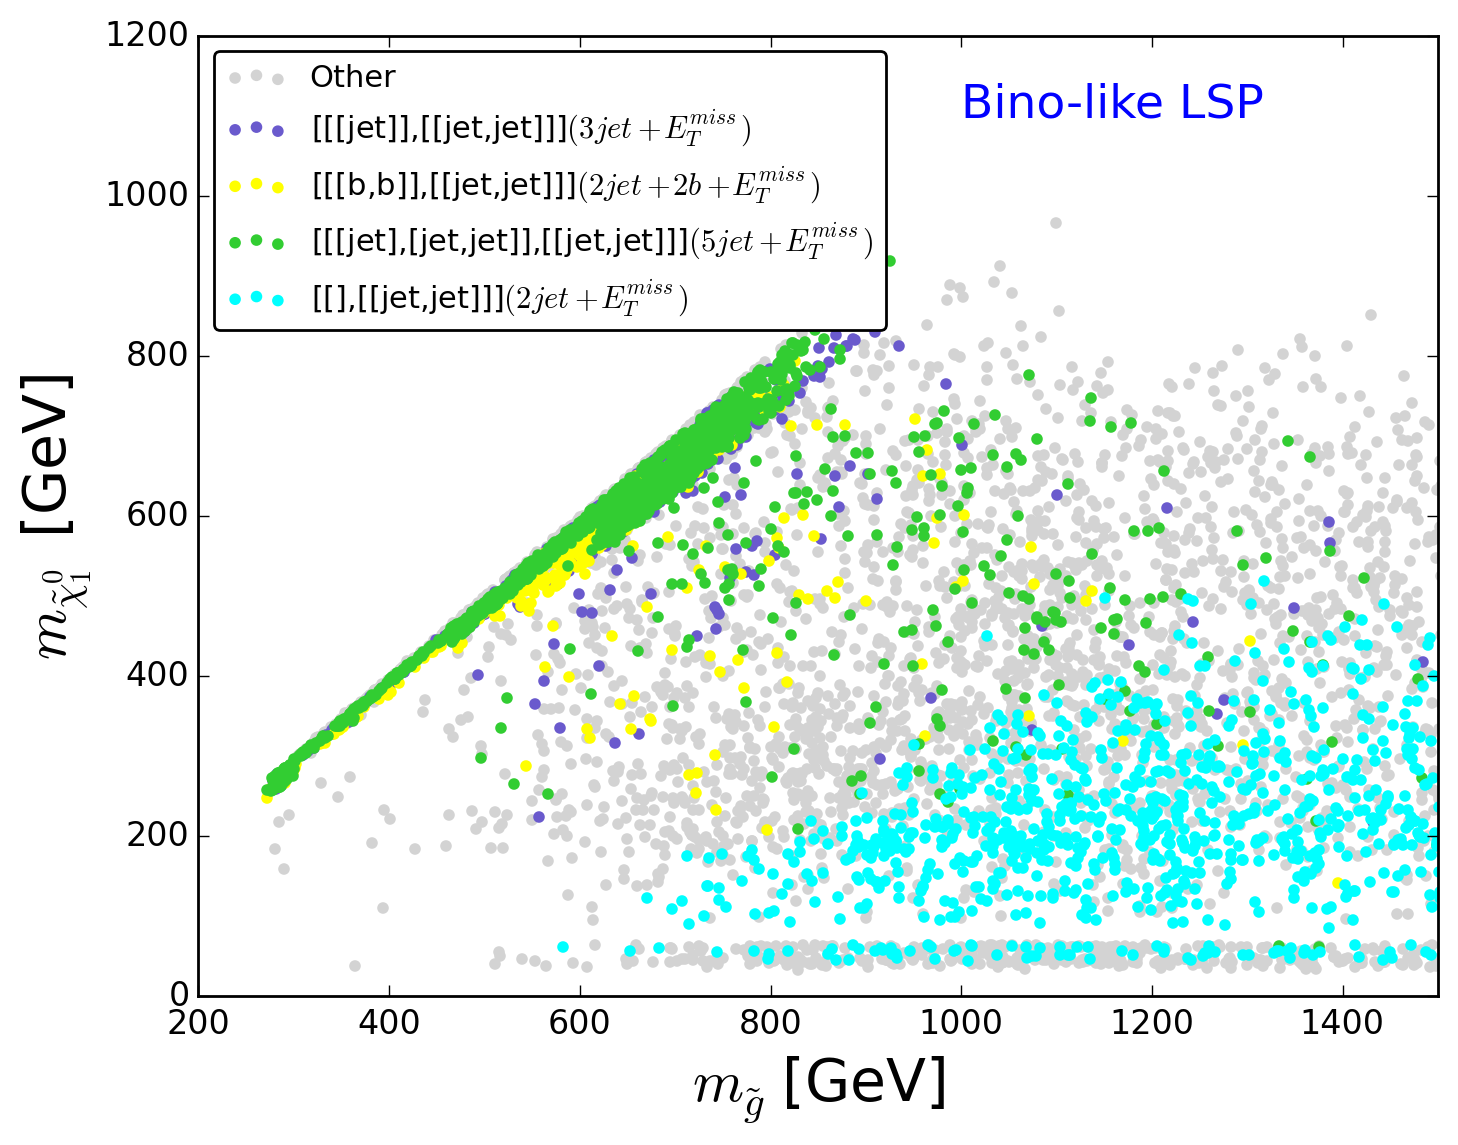
\includegraphics[width=0.49\textwidth]{PLOTS/Missing/BINO_Zoom_Missing_GluNeu.png}}
%\end{center}
%\caption{Missing topologies with the highest weights for the Bino-like LSP dataset.} 
%\label{Missing_Bino}
%\end{figure}
%
%\begin{figure}[!]
%\begin{center}
%\subfigure
%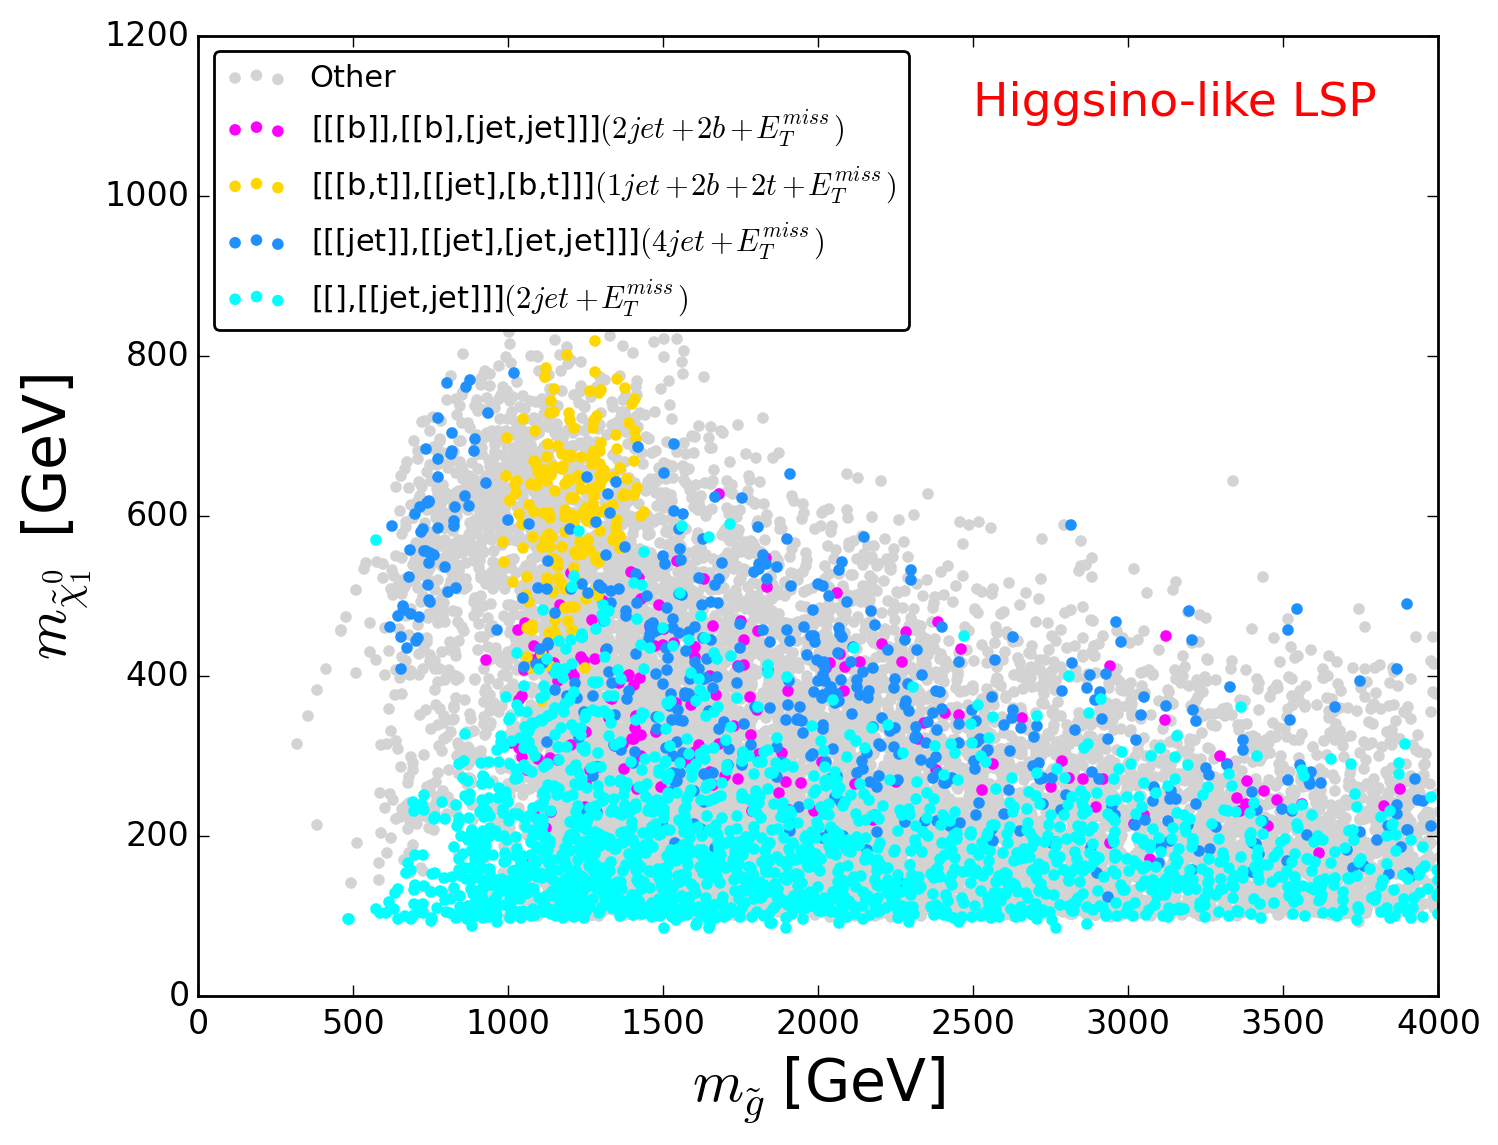
\includegraphics[width=0.49\textwidth]{PLOTS/Missing/HIGGSINO_Missing_GluNeu.png}
%\subfigure
%{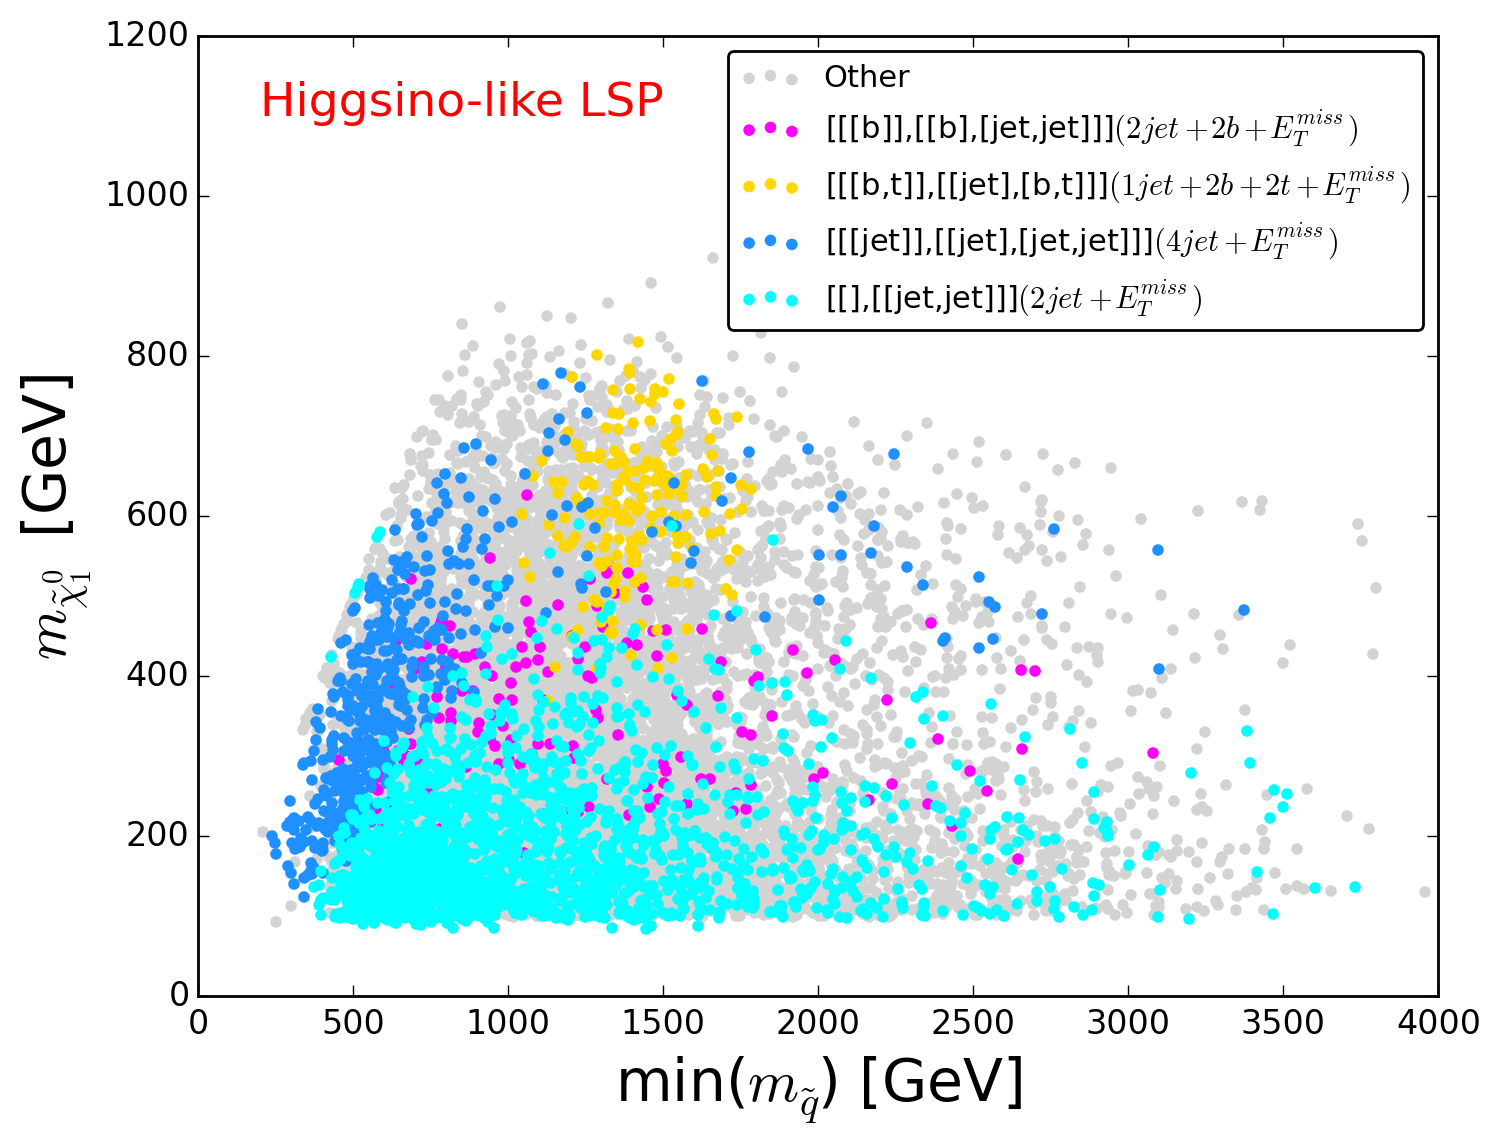
\includegraphics[width=0.49\textwidth]{PLOTS/Missing/HIGGSINO_Missing_SqNeu.png}}
%\subfigure
%{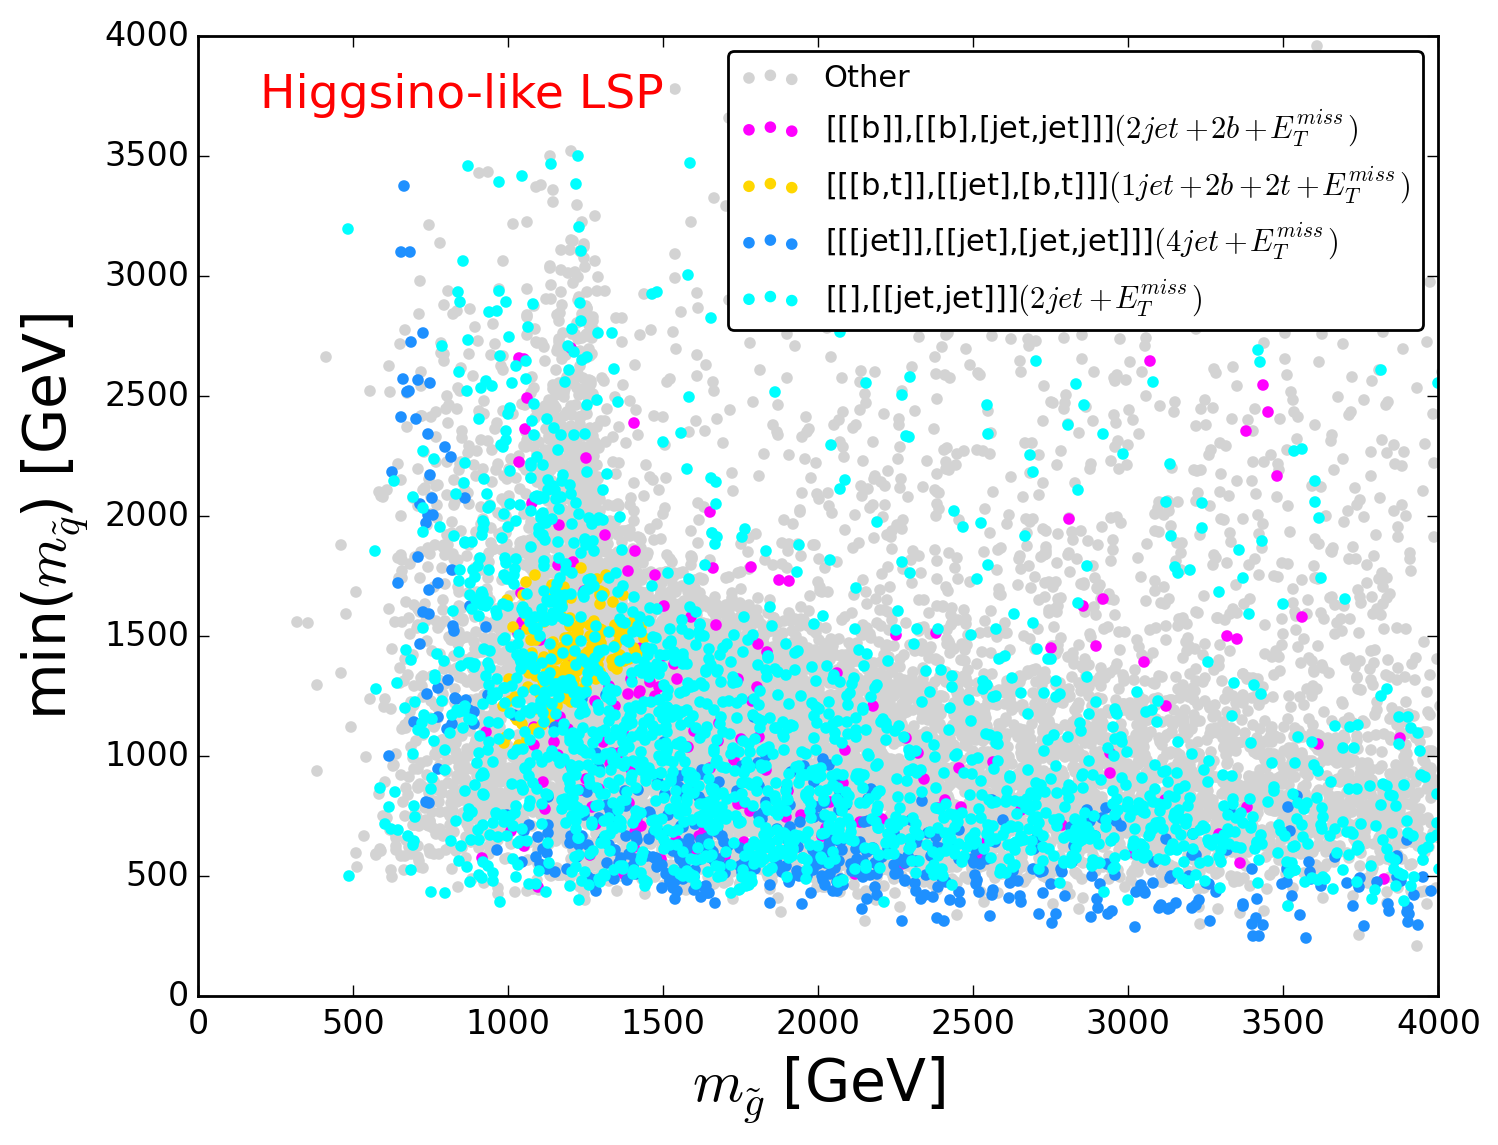
\includegraphics[width=0.49\textwidth]{PLOTS/Missing/HIGGSINO_Missing_GluSq.png}}
%\subfigure
%{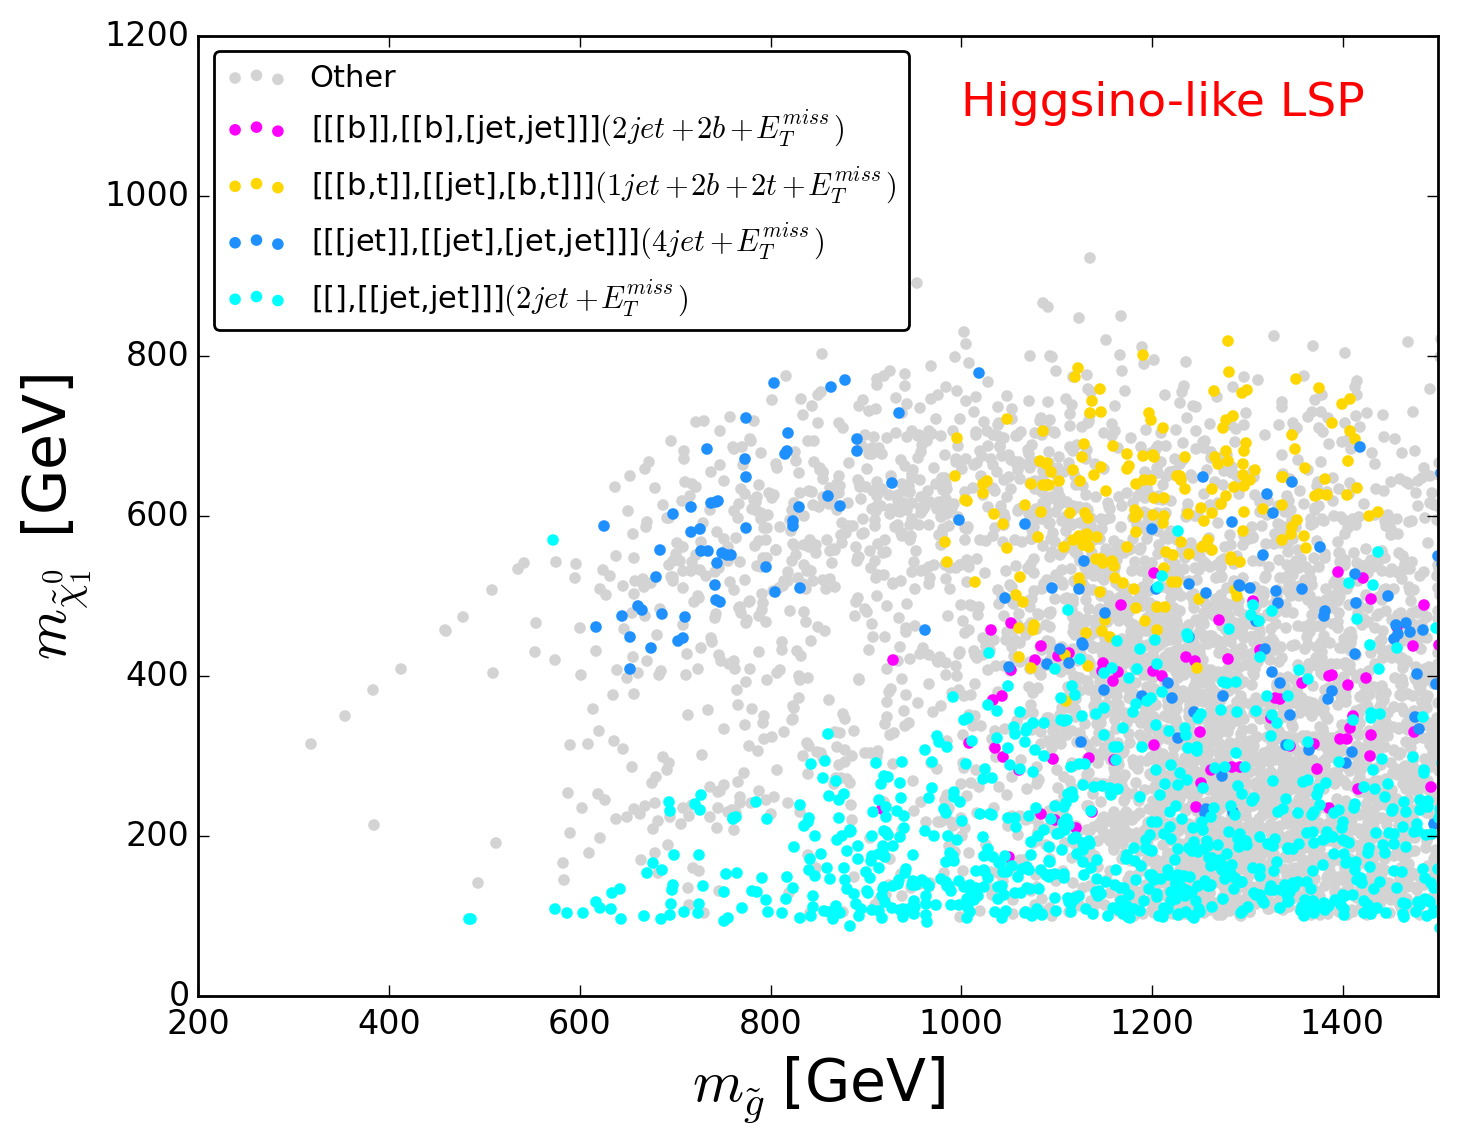
\includegraphics[width=0.49\textwidth]{PLOTS/Missing/HIGGSINO_Zoom_Missing_GluNeu.png}}
%\end{center}
%\caption{Missing topologies with the highest weights for the Higgsino-like LSP dataset.} 
%\label{Missing_Higgsino}
%\end{figure}
%
%\section{Comparison with 13 TeV Results}
%
%In general it is believed that the latest results from the LHC experiments, obtained with data collected at 13 TeV centre-of-mass energy, provide better limits with respect the analogous results obtained by previous 8 TeV searches. Besides an improvement in the collision energy, recent searches are also based on larger dataset, due to a large integrated luminosity wrt Run 1. In the context of simplified models, however, such belief is not totally justified, depending primarily on the type of simplified model that are used for the interpretation of the searches. Besides few results provided by the ATLAS collaboration, see e.g. {\color{blue} to do}, in the form of efficiency maps, only upper limit results are available, relative to limited variety of simplified models. It is interesting then to investigate if there are pMSSM points that can be excluded at 8 TeV thanks to the \TGQ~homegrown results, but that survive 13 TeV constraints with the available simplified models. Table \ref{13_TeV} summarises the number of points that cannot be excluded with 13 TeV results. 
%
%\begin{table*}
%\center
%\renewcommand{\arraystretch}{1.3}
%\begin{tabular}{ l | c   c  }
%\textbf{Number of Points} & \textbf{Bino-like LSP }& \textbf{Higgsino-like LSP} \\
%\toprule \toprule
%Non Decoposed  & 256 & \\
%Non Excluded & 262  &  { \color{blue} xxx } \\
%Total Non Constrained  & 518 & \\
%\\ 
%\hline
%\end{tabular}
%\caption{Summary of points excluded by the newly added 8 TeV EMs results, that cannot be excluded at 13 TeV (see text for details about the 13 TeV results considered.} }
%\label{13_TeV}
%\end{table*}
%{\color{blue} Ideally, make a cmparison with the T2 results *only*} 
\section{A Look at 13 TeV Results}\label{ch::13TeV}
In this Section we discuss briefly what happens with SMS results produced with 13 TeV centre-of-mass energy collision data. Due to the large increase in the production cross section, it is expected that the coverage of the pMSSM-19 for the same dataset of points designed for 8 TeV results, increases considerably. In fact, this was already shown in \cite{Dutta:2018ioj}: by using SMS results for a selection of 13 TeV analyses, with collision data adding up to around 36 $fb^{-1}$, almost all the entire set of pMSSM-19 points considered by ATLAS could be excluded, including the ones out of the of 8 TeV searches, mainly due to very small values of the cross sections. The aim of the present discussion is to demonstrate that, despite the large increase in the production cross section, certain regions of the parameter space cannot be covered even with the latest results. 
\\

%
\begin{figure}
	\begin{center}
		\subfigure
		{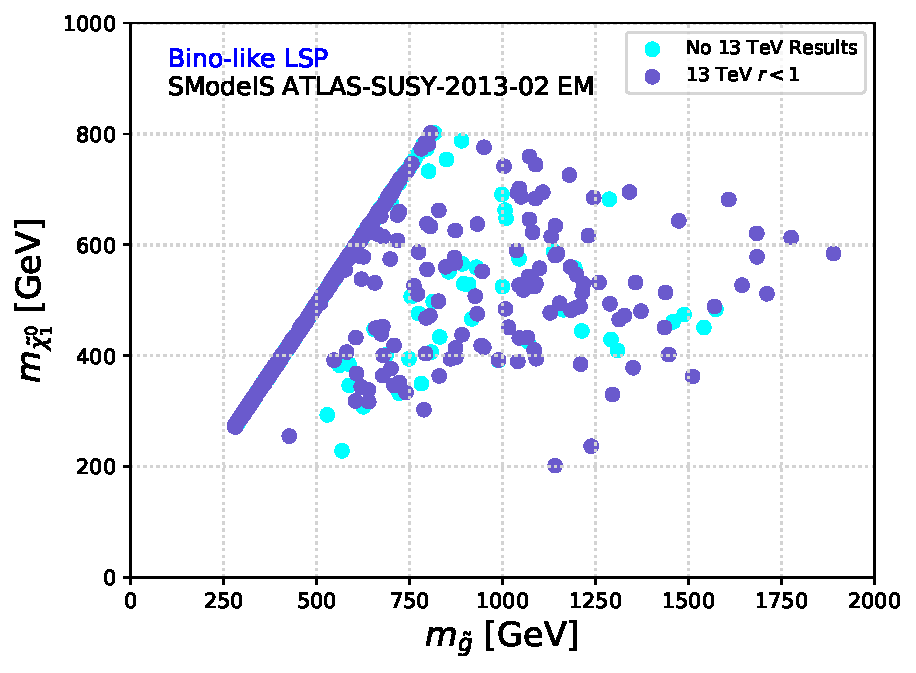
\includegraphics[width=0.49\textwidth]{PLOTS/13TeV/13TeV_Glu_Neu.pdf}}
		\subfigure
		{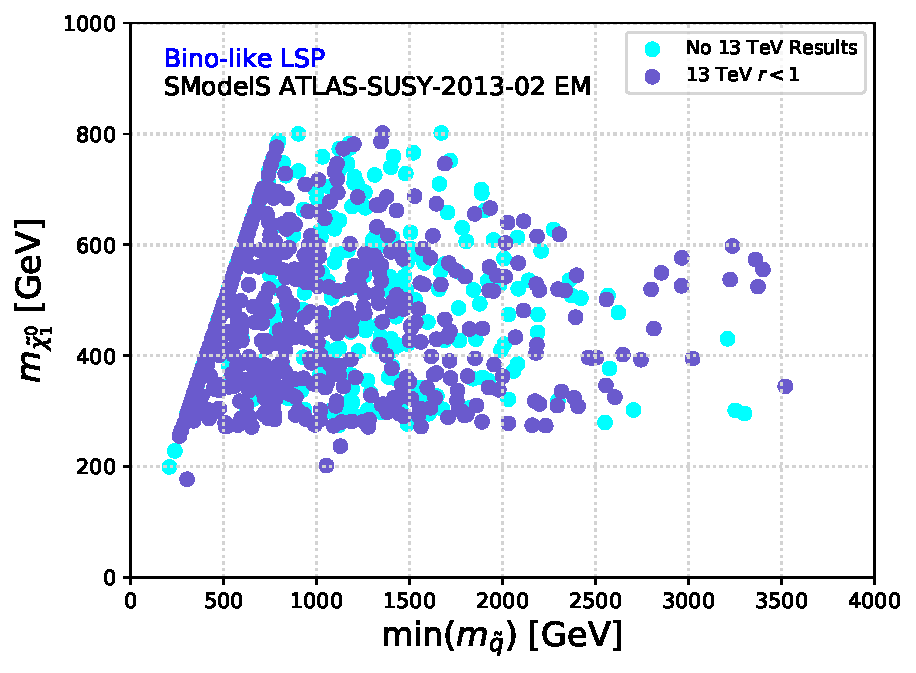
\includegraphics[width=0.49\textwidth]{PLOTS/13TeV/13TeV_Sq_Neu.pdf}}
	\end{center}
	\caption{Distribution of the points (Bino-like LSP dataset) excluded by the 8 TeV EM results for the analysis ATLAS-SUSY-2013-02, but not excluded by recent 13 TeV analyses published in v1.2.2 of the \SMO~ database. In cyan, the points fall outside the grid of results available for 13 TeV results; in purple, points for which the 13 TeV $r \ value <1$. Note that most of the points lies in the region of small gluino/squark-LSP mass gap.}. 
	\label{13TEV}
\end{figure}
%
%
In Fig. \ref{13TEV} we consider a set of points which can be excluded with the new ATLAS-SUSY-2013-02 EMs, but cannot be excluded by the 13 TeV results implemented in the most updated release v.1.2. of the \SMO~ database. The points are divided into two categories. The first include points that do not map onto any of the available results, mainly because the mass array characterising the models in the decomposition cannot be mapped onto the mass grid of the results. The second category includes points for which 13 TeV results can indeed be applied, but they prove insufficient to exclude the points. 
The two different mass planes show clearly that indeed the majority of points falls in the region where the mass gap between the gluino-LSP or squark-LSP is small. In Fig. \ref{13TeVrvalue} we also include the distributions of 8 TeV ATLAS-SUSY-2013-02 results, which reaches up to values greater than few tens.
%
We note that the recent Run 2 inclusive ATLAS 0 lepton,2-6 jets search\cite{Aaboud:2017vwy}, that uses 36 $fb^{-1}$ of collision data, is interpreted with gluino and squark pair production and gluino-squark SMS. In particular, the gluino-squark model is in fact a realisation of the pMSSM where only 1st and 2nd generation squarks and gluinos are considered, and all the other sparticles are decoupled. They parametrized the mass planes by fixing the LSP mass (Bino-like, for $m_{\tilde \chi _1} ^0 = (0,695,995)$ and considered a grid of gluino and squark masses. We note that the in order to use such results, an interpolation in the LSP mass of around 700 GeV, to cover the region $m_{\tilde \chi _1} ^0 < 700$ GeV , has to be performed. Unfortunately the results are provided (on \texttt{InspireHEP}\cite{HEP201607} only in the form of UL maps. It would be much appreciated if EMs for the gluino-squark model were also made available and allow for the combination with the published EMs for the \Ttwo~model. 
%
%
%
\begin{figure}
	\begin{center}
		
		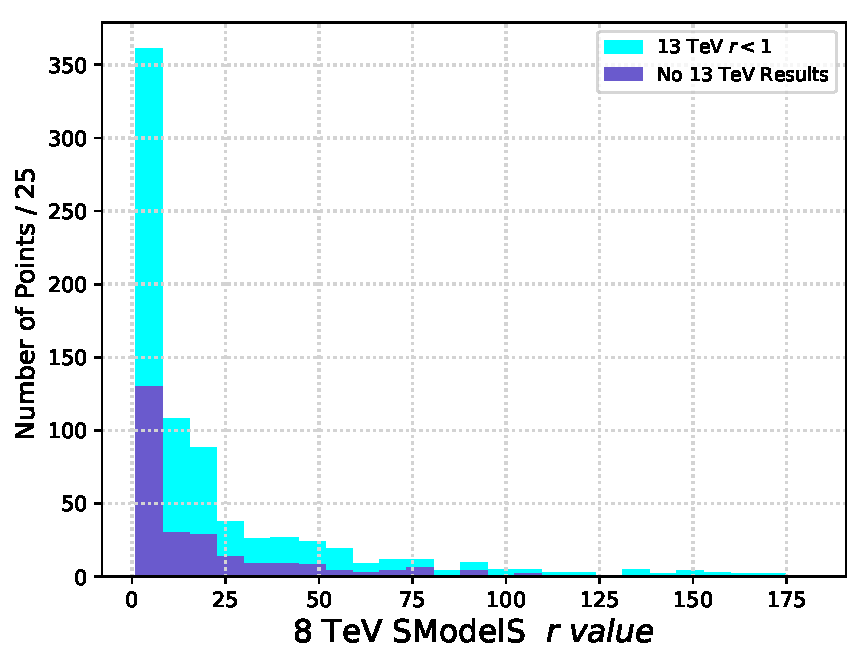
\includegraphics[width=0.49\textwidth]{PLOTS/13TeV/rvalues.pdf}
		
	\end{center}
	\caption{Distribution of points (Bino-like LSP dataset) excluded by the 8 TeV EM results for the analysis ATLAS-SUSY-2013-02, but not excluded by recent 13 TeV analyses published in v1.2.2 of the \SMO~ database. In cyan, the points fall outside the grid of results available for 13 TeV results; in purple, points for which the $r \ value <1$ with 13 TeV results. Note that most of the points lies in the region of small gluino/squark-LSP mass gap.}. 
	\label{13TeVrvalue}
\end{figure}
Finally, we provide the results of one of such points, the SLHA file \textit{59847871} from the Bino-like LSP dataset. The mass spectrum, adapted from the tool \texttt{pySLHA}\cite{Buckley:2013jua}, is shown in Fig. \ref{pyslha}. We see that, besides the light neutralinos/chargino $\tilde \chi _1 ^0,\tilde \chi _2 ^0,\tilde \chi _3 ^0,\tilde \chi _1 ^{\pm}$ whose mass lies around 500 GeV, the lightest SUSY particles are down-type right-handed squark, with mass of 854 GeV. The gluino is slightly heavier, with a mass of 1.072 TeV. The up-type right-handed and the left-handed squarks have a mass of 1.763 and 2.353 TeV respectively. In Table \ref{tab_13tev} the results from the best 13 TeV analysis and the results from our recast EMs for the 8 TeV searches are shown, and the values for the production cross section in Tab. \ref{cross_sections}. 
%
%
\begin{figure}
	\begin{center}		
		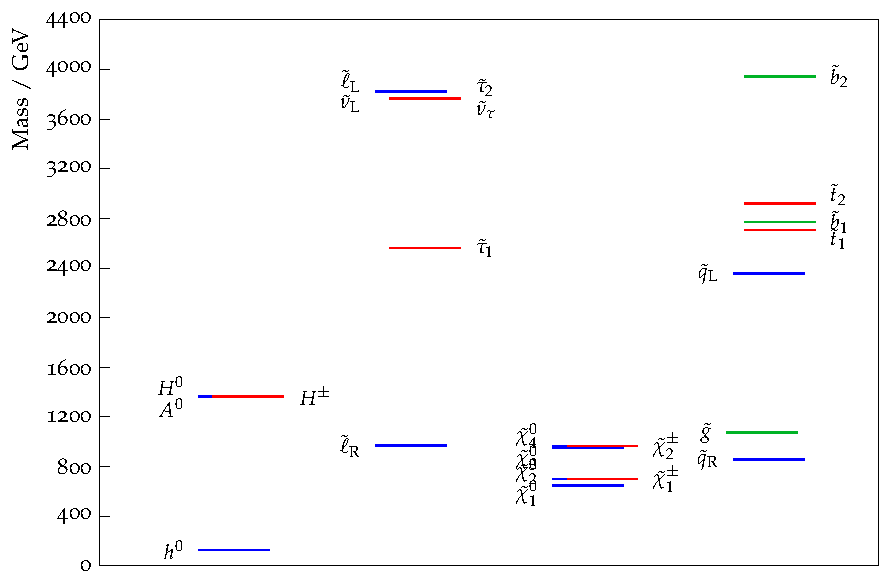
\includegraphics[width=0.49\textwidth]{PLOTS/13TeV/59847871.pdf}
	\end{center}
	\caption{Mass spectrum of the point \textit{59847871}, from the Bino-like LSP dataset. Right-handed squarks are the lightest coloured particles, opening the $\tilde g \rightarrow q \tilde q $ decay channel. {\color{blue} FIX!!! right up and down squarks}} 
	\label{pyslha}
\end{figure}
%
%

\begin{table}[!h]
	\footnotesize
	\begin{center}
		\renewcommand{\arraystretch}{1.3}
		\begin{tabular}{ l c c}  \toprule \toprule
			\multicolumn{3}{c}{Point 59847871 Bino-like LSP dataset} \\ \toprule 
			\textbf{Analysis} & \textbf{$\sqrt{s}$ [TeV]}  & \textbf{r value} \\  \toprule
			ATLAS-SUSY-2013-02 (EM) & 8.0  &  1.57 \\
			CMS-SUS-16-033 (UL) & 13.0 & 0.79 \\
			CMS-SUS-16-036 (UL) & 13.0 & 0.69 \\
			\bottomrule
		\end{tabular}
	\end{center}
	\caption{Results of the analysis of the point 59847871 Bino-like LSP dataset, showing the analyses with the top three \RVALUE. }
	\label{tab_13tev}
\end{table}
%
%
\begin{table}[!h]
	\footnotesize
	\begin{center}
		\renewcommand{\arraystretch}{1.3}
		\begin{tabular}{ l c c}  \toprule \toprule
			\textbf{Process} & $\sigma$(8 TeV) [pb]  & $\sigma$(13 TeV) [pb] \\  \toprule
			$pp \rightarrow \tilde g \tilde g$ & 1.09*10$^{-2}$ & 1.66*10$^{-1}$\\
			$pp \rightarrow \tilde g \tilde q$ & 1.01*10$^{-2}$ &  2.9*10$^{-1}$ \\
			$pp \rightarrow \tilde q \tilde q$ & 1.67 10$^{-2}$ & 8.84*10$^{-2}$ \\
			\bottomrule
		\end{tabular}
	\end{center}
	\caption{Cross section production [pb] for the processes $pp \rightarrow \tilde g \tilde g$,$pp \rightarrow \tilde g \tilde q$, $pp \rightarrow \tilde q \tilde q$. Cross sections values are calculated at NLL order.}
	\label{cross_sections}
\end{table}




\section{Conclusion}\label{sec:conclusion}
While simplified models have become hugely popular among the experimental collaboration for the interpretation of their BSM searches, it is always challenging to make use of such results to investigate complicated theories. Moreover, the question if the simplified approach is sufficient to properly cover the a full model is always open. A concrete step forward was made by analysing the ATLAS pMSSM-19 dataset with simplified models, showing that a large portion of the parameter space of such SUSY model can be efficiently constrained by means of SMS, without the computationally expensive procedure of analyses recasting. At the same time,  despite the plenty SMS results, there is a lot of room for improvement in the coverage. The essence of SMS makes them inadequate in the presence of  complicated mass spectra, that give rise to long decay patterns and that are better captured by full analyses recast. Fortunately the main outcome of the previous study showed clearly that for the majority of uncovered model points, most of the unconstrained $\sigma \times BR$ was captured by a class of simplified models involving only three SUSY particles and short decay, arising from gluino-squark production. The associated $3jets+$\MET~ signature is easily covered by inclusive all hadronic final state searches at the LHC, targeting specifically low jet multiplicity, such as ATLAS-SUSY-2013-02 and CMS-SUS-13-012. The results presented in this work show concretely that it is possible to produce such dedicated EM results, using available recasting tools, and significantly increase the coverage of the model up to 74$\%$ and 71$\%$ of the total ATLAS exclusion for the Bino and Higgsino like LSP dataset respectively. 
Moreover, due to the large cross section for gluino-squark production, it was shown that the new EMs could be still extended to larger particle mass, and obtain additional constraints. 
The workflow can be extended and implemented for other theories: once the most important missing simplified signatures are determined, recast EM can be produced only once, and the results can be re-used to constrain generic models. In addition to the possibility to produce customized SMS results, EMs have the advantage of allowing the combination of multiple signals. In particular, the combination of the \Ttwo+\Tfive+\TGQ~signals for the ATLAS-SUSY-2013-02 analysis is sufficient to cover the XX and XX of the points covered by the full recast of the analysis, as performed by ATLAS. We note that this is obtained by neglecting most of the popular simplified model for gluino production, such as the direct decays of gluinos via off-shell top $pp \rightarrow \tilde g \tilde g, \tilde g \rightarrow t \bar t \chi _1 ^0$ and sbottom squarks $pp \rightarrow \tilde g \tilde g, \tilde g \rightarrow b \bar b \chi _1 ^0$, and models for third generation squarks direct decay such as $pp \rightarrow \tilde b \tilde b, \tilde b \rightarrow b \chi _1 ^0$ and $pp \rightarrow \tilde b \tilde b, \tilde b \rightarrow b \chi _1 ^0$, to which the search is expected to be sensitive to (see e.g. \cite{Kraml:2016eti} for the top squark model). 
On another note, we are aware that the latest data, referring to proton collisions at 13 TeV centre-of-mass energy, give much better constraints on the same model due to the significant increase in the production cross section, and also in the larger amount of data, since the latest SUSY searches form the ATLAS and CMS collaborations are based on an integrated luminosity of around 140 $fb^{-1}$, already a factor 7 higher than the luminosity collected during Run 1. The impact on the pMSSM-19 was already estimated in \cite{Dutta:2018ioj}. There is however a substantial difference and outcome in the aim of the two works. With this study, we aimed at somehow give a concrete exemplification of systematic use of the tool \SMO~ in association with public recasting tool to improve what is the state of the art of the available SMS results. Stressing the importance of specific simplified models results, produced for specific SUSY searches, is valuable information for the future. In fact, still neither the \Tfive nor the \TGQ models are available at higher centre-of-mass energy, being those official or recast results. This works constitute a solid starting point for building future updates of the databases of SUSY SMS results, and we invite both the experimental collaboration and our colleague phenomenologists to produce UL and/or EM results for the SMS here studied.
%
\section*{Acknowledgments}
The author thanks Wolfgang Waltenberger, Sabine Kraml, Ursula Laa and Andre Lessa from the SModleS collaborations for useful discussions, and for providing the data used in the comparison with early 13 TeV results. The author is grateful to the Institut f\"ur Hochenergiephysik of the \"Osterreichische Akademie der Wissenschaften for the opportunity to use the computing facilities.
%
\bibliography{references}
\addcontentsline{toc}{section}{References}
\bibliographystyle{JHEP}
\clearpage
\appendix
%
\section{Limits Comparison}\label{app:ul}
Tables \ref{ATLAS02_UL} and \ref{ATLAS02_UL_2}  compare the upper limits obtained for the mass point ($M_1,M_2,M_3) = (1000,200,190),(1200,600,500)$ GeV for the two different hierarchy models \textit{T3GQ}($m_{\tilde g}, m_{\tilde q}, m_{\tilde \chi _1 ^0 }$) and \textit{T3QG}($m_{\tilde q}, m_{\tilde g}, m_{\tilde \chi _1 ^0 }$). In bold, the best SR providing the strongest expected limit and corresponding observed limit is shown. The difference in the efficiency and consequent choice of a different SR, respectively \textit{2jm} for \textit{T3GQ} and \textit{2jt} for \textit{T3QG}, favours a strongest limit for the \textit{T3GQ} case. However the difference is contained within a factor 2, which translates to only few tens of GeV difference in the excluded mass of Squarks or Gluinos. The value of the observed UL, quoted by \SMO, is indicated with an asterisk. 
\begin{table*}[h]
	\centering
	\renewcommand\arraystretch{1.3} 
	\scriptsize
	\begin{tabular}{ l c c    c c c  |  c c c  }
		\toprule \toprule
		\multicolumn{3}{c}{($M_1,M_2,M_3) = (1000,200,190)$} & \multicolumn{3}{c}{ \textbf{T3GQ}} & \multicolumn{3}{c}{ \textbf{T3QG}} \\  \toprule 
		\textbf{SR} & $UL_{exp}$ & $UL_{obs}$ & $\epsilon$ &  $UL_{exp}/\epsilon$ & $UL_{obs}/\epsilon$ & $\epsilon$ & $UL_{exp}/ \epsilon$ & $UL_{obs}/ \epsilon$ \\
		2jm & 5.552 &  4.242 &  0.118  & \textbf{47.1} &  \textbf{36.0}  &  0.090 &  \textbf{61.5}*  & \textbf{47.0}*\\
		2jt  & 1.512  & 1.818 &  0.032  & \textbf{47.9} &  \textbf{57.5}  &  0.027 &  \textbf{56.1}  & \textbf{67.4} \\
		3j &  0.332 &  0.433  & 0.002 &  139.4 &  182.2  &  0.002 &  186.4 &  243.6 \\ 
		4jl  & 5.435 &  4.749  & 0.032  & 171.4  & 149.8  &  0.039 &  139.7  & 122.1 \\
		4jl-  & 11.561 &  13.292 &  0.036  & 318.7 &  366.4  &  0.047 &  248.0 &  285.2 \\
		4jt  & 0.240  & 0.149  & 0.002  & 146.1  & 90.8 &   0.001  & 178.1  & 110.8 \\
		5j  & 1.714  & 1.543  & 0.007 &  245.1 &  220.7  &  0.010  & 172.9  & 155.6 \\
		6jl  & 1.531  & 1.923  & 0.002  & 965.5 &  1212.5  & 0.003  & 555.5 &  697.7 \\
		6jt &  0.333  & 0.332 &  0.001  & 472.8  & 470.4 &  0.001 &  327.8  & 326.2 \\
		6jt+  & 0.302 &  0.399 &  0.001  & 428.6  & 566.3  & 0.001  & 297.2  & 392.7 \\
		\bottomrule \bottomrule
	\end{tabular}
	\caption{Summary of the UL for the SRs of ATLAS-SUSY-2013-02, for the \textit{T3GQ} and \textit{T3QG} models, with mass spectrum ($M_1,M_2,M_3) = (1000,200,190)$ GeV. In bold, the expected and observed limits for the best SRs are highlighted. With a star, the value of the observed UL used by \SMO~ is indicated.}
	\label{ATLAS02_UL}
\end{table*}
\begin{table*}[h]
	\centering
	\renewcommand\arraystretch{1.3} 
	\scriptsize
	\begin{tabular}{ l c c    c c c  |  c c c  }
		\toprule \toprule
		\multicolumn{3}{c}{($M_1,M_2,M_3) = (1200,600,500)$} & \multicolumn{3}{c}{ \textbf{T3GQ}} & \multicolumn{3}{c}{ \textbf{T3QG}} \\  \toprule 
		\textbf{SR} & $UL_{exp}$ & $UL_{obs}$ & $\epsilon$ &  $UL_{exp}/\epsilon$ & $UL_{obs}/\epsilon$ & $\epsilon$ & $UL_{exp}/ \epsilon$ & $UL_{obs}/ \epsilon$ \\
		2jm & 5.552 &  4.242 &  0.178	 &31.172 &	23.815		 &0.184	 &30.111	 &23.004 \\
		2jt  & 1.512  & 1.818 &  0.061& 	\textbf{24.623}	& \textbf{29.601}	& 	0.069	& \textbf{21.949}*& 	\textbf{26.385}* \\
		3j &  0.332 &  0.433  & 0.005& 	61.421& 	80.255		& 0.005	& 64.971& 	84.893 \\ 
		4jl  & 5.435 &  4.749  & 0.165	& 69.892	& 80.356	& 	0.188	& 61.542& 	70.756  \\
		4jl-  & 11.561 &  13.292 &  0.145	& 37.596	& 32.851		& 0.166	& 32.813	& 28.672 \\
		4jt  & 0.240  & 0.149  & 0.004& 	54.035	& 33.611		& 0.004	& 54.765& 	34.065  \\
		5j  & 1.714  & 1.543  &0.048	& 36.043	& 32.449	& 	0.055	& 31.004	& 27.912  \\
		6jl  & 1.531  & 1.923  & 0.016	& 98.361	& 123.530	& 	0.018	& 83.039	& 104.286 \\
		6jt &  0.333  & 0.332 &  0.008	& 43.713& 	43.489	& 	0.007	& 45.136	& 44.905  \\
		6jt+  & 0.302 &  0.399 & 0.008& 	39.632& 	52.359	& 	0.007	& 40.922	& 54.063 \\
		\bottomrule \bottomrule
	\end{tabular}
	\caption{Summary of the UL for the SRs of ATLAS-SUSY-2013-02, for the \textit{T3GQ} and \textit{T3QG} models, with mass spectrum ($M_1,M_2,M_3) = (1200,600,500)$ GeV. In bold, the expected and observed limits for the best SR are highlited.}
	\label{ATLAS02_UL_2}
\end{table*}

\section{Distributions of r values}
Fig.\ref{Histos_r} shows the distributions of the $r$ values for each result of the analysis ATLAS-SUSY-2013-02 (\textit{T1},\textit{T2},\textit{T5} and \textit{T3GQ}), the combinations of models (\textit{T2+T5}, \textit{T2+T5+T3GQ} and the sum of all the available results \textit{T1+T2+T5+T3GQ}). Only the points excluded by the analysis are considered; this implies that the points in the first bin $0\leq r < 1$ can be excluded only by considering the sum of all the results, i.e. considering \textit{T1+T2+T5+T3GQ}. For the bins with $r \geq 1$, each individual contribution might be sufficient to exclude the models tested. For large rvalues, the number of points decreases as expected, and the importance of the combinations of multiple results increases. The last bin refers to $rvalue \geq 10$, i.e. points that can be strongly excluded by the SMS results considered, in particular by the combination of the \textit{T1+T2+T5+T3GQ} and \textit{T2+T5+T3GQ} for the Bino and Higgsino-like LSP case respectively. 
\begin{figure}[!h]
	\begin{center}
		\subfigure
		{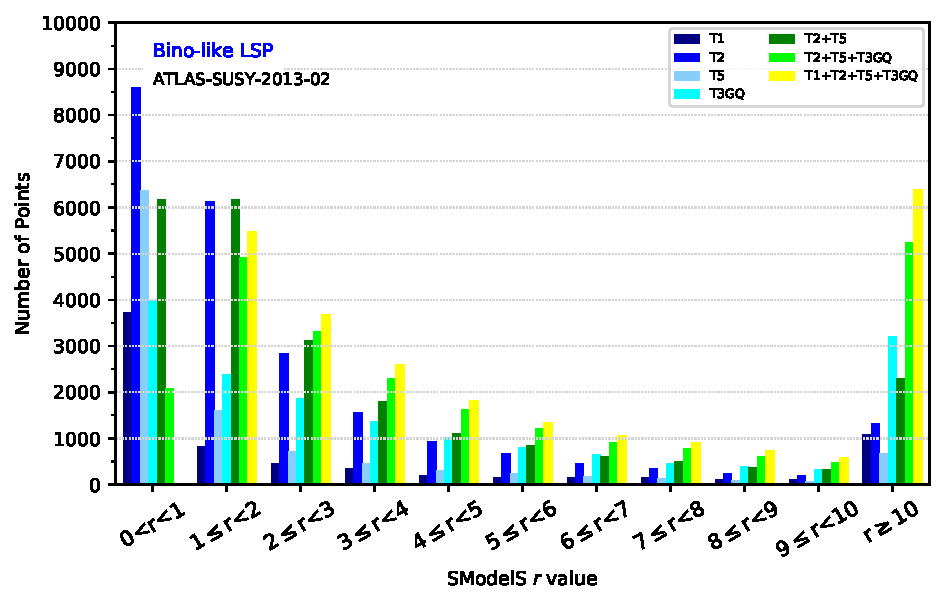
\includegraphics[width=0.49\textwidth]{PLOTS/Combination/ATLAS-SUSY-2013-02_Bino_rValuesHisto.pdf}}
		\subfigure
		{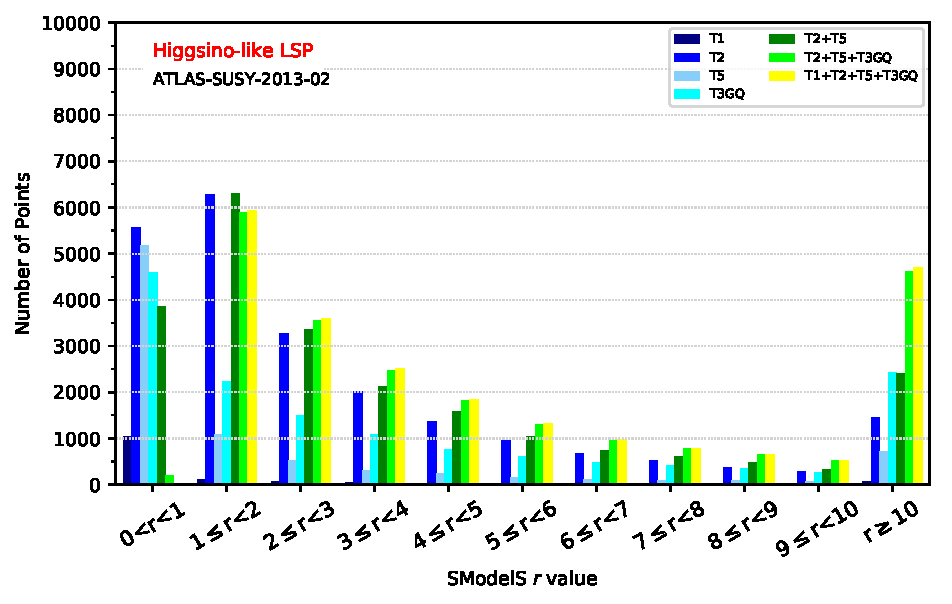
\includegraphics[width=0.49\textwidth]{PLOTS/Combination/ATLAS-SUSY-2013-02_Higgsino_rValuesHisto.pdf}}
	\end{center}
	\caption{Distribution of the $r$ values for excluded points, considering single SMS or combinations, for the analysis ATLAS-SUSY-2013-02. The points included in the first bin $0<r \ value < 1$ can only be excluded by the combination of all the EMs results available for the ATLAS-SUSY-2013-02 analysis.} 
	\label{Histos_r}
\end{figure}


%
%\bibliographystyle{JHEP}
%\bibliography{references}
%\bibliographystyle{utphys.bst}
\end{document}



